\section{设计过程}
\subsection{设计流水账}
2023年12月25日:胡欣凯、李宽宇根据lab4初始化mycpu;

2023年12月25日:胡欣凯、李宽宇运行lab4;

2023年12月25日:胡欣凯SignExtend更改为DataExtend。新的控制器信号ImmSignE用于确定是否使用SignImmE或UnsignImmE。适用于ANDI,XORI,LUI,ORI。李宽宇添加算术指令和位移指令。

2023年12月26日:胡欣凯通过了$Lab4$的回归测试。

2023年12月27日:胡欣凯、李宽宇调整了代码格式。

2023年12月29日:胡欣凯通过了lab4测试,通过了 ArthmeticTest (除了DIV和DIVU), DataMoveInstTest, LogicInstTest, ShiftInstTest,在 jBTest 中失败。

2023年12月31日:除( DIV , save and load)外的所有基本指令都已通过和检查。 DIV 在 DivStall 上有些问题。

2024年1月1日: save 和 load 指令完成。所有52条基本指令已完成。胡欣凯添加了调试注释。

2024年1月1日:修复了除数和 hilo 寄存器中的错误。李宽宇添加了代码注释。

2024年1月2日:修复了save 和 load 指令完成的错误。

2024年1月3日:完善了访存指令和冒险,添加了 cp0 和 exception 指令。几乎完成了57条指令。

2024年1月3日:连接了带有错误的SRAM接口。

2024年1月5日:通过了所有89个功能测试。

2024年1月7日:通过了76个与AXI接口相关的功能测试。

2024年1月8日:AXI功能测试通过。

2024年1月9日:通过了性能测试。

2024年1月9日:修复了cache中的错误。

2024年1月10日:改进了cache。

\subsection{错误记录}

\subsubsection{错误1}
\begin{enumerate}[(1)]
    \item 错误现象

在对分支跳转指令单独进行测试时,观察到结果 ResultW 未出现 0xa 以后的数字。正确现象为 ResultW 中依次出现从 0x1 到 0x14 的数字。

\begin{figure}[H]
    \centering
    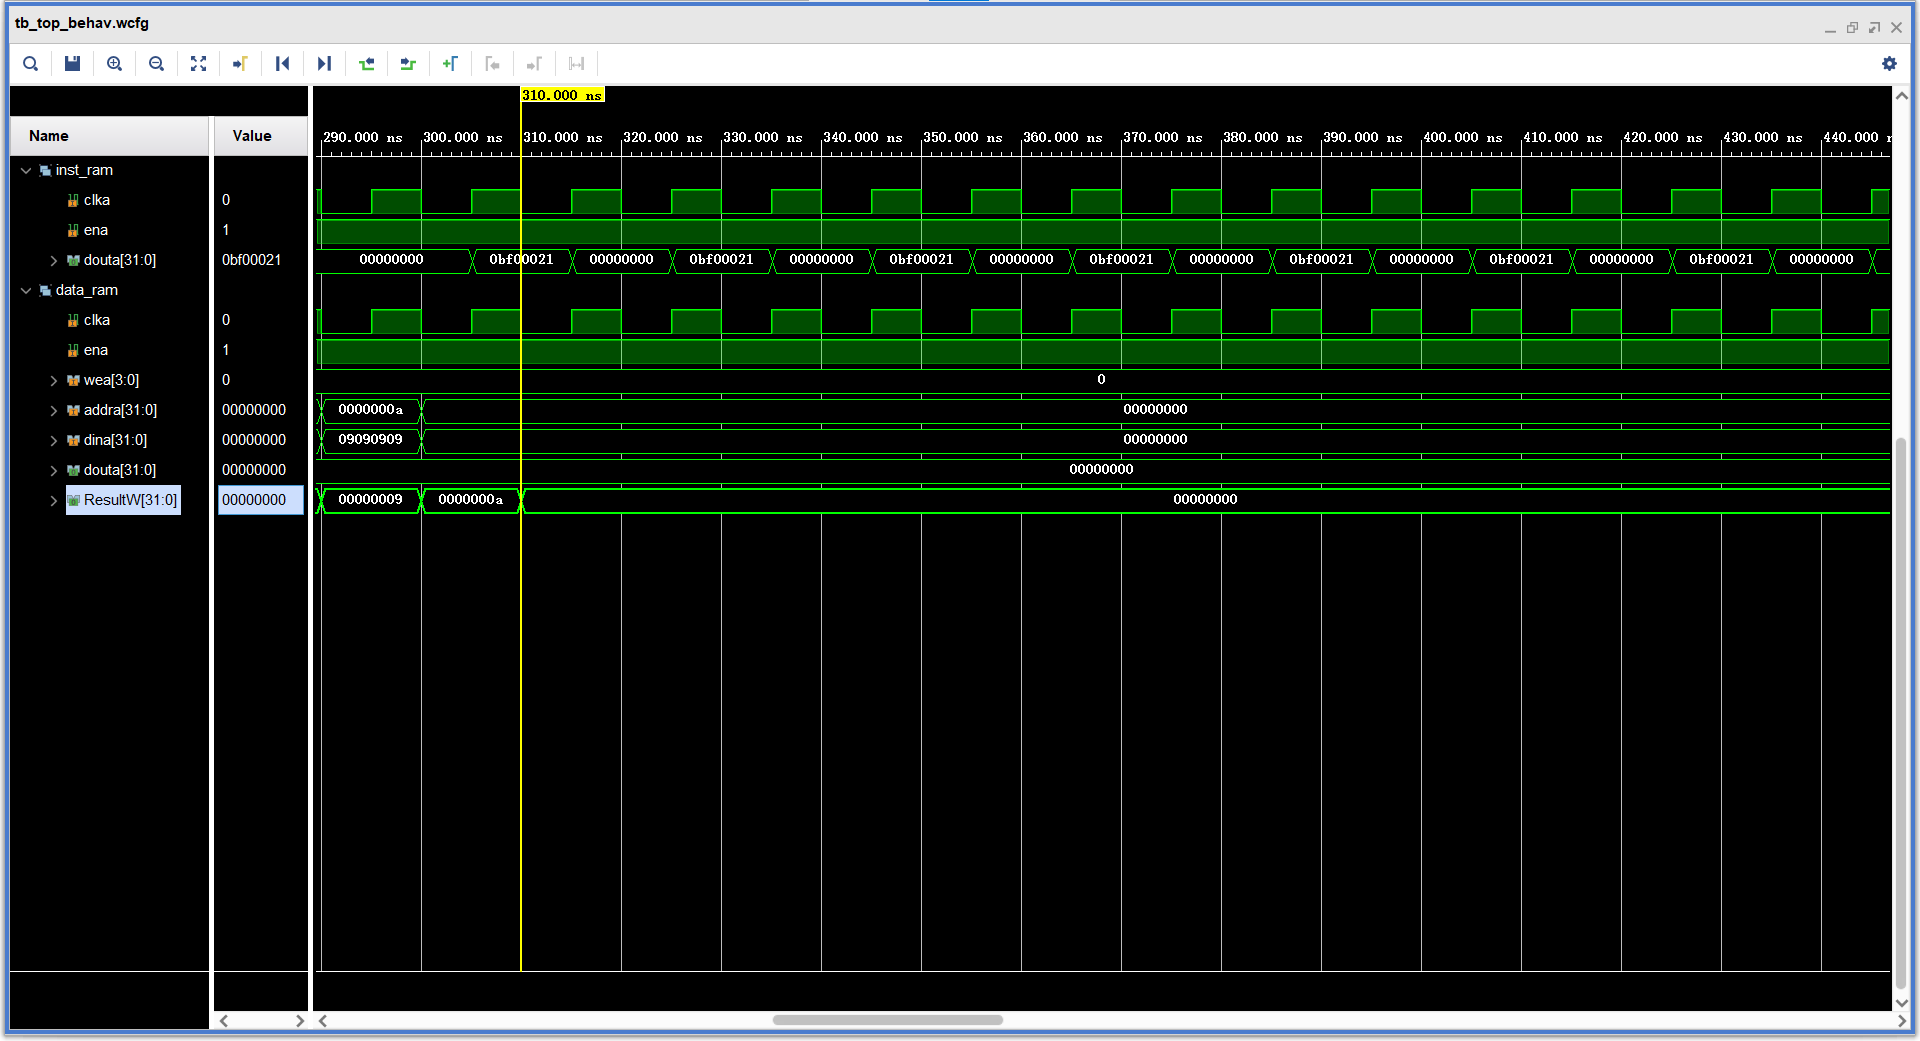
\includegraphics[width=\textwidth]{image/错误1-错误现象1.png}
    \caption{错误1-错误现象:ResultW 未出现 0xa 以后的数字}
    \label{fig:错误1-错误现象1}
\end{figure}

    \item 分析定位过程

由于分支指令与 PCSrcD 信号相关,因此查看该信号的变化。观察到 PCSrcD 有 4 次值为 1,即仅跳转 4 次。

\begin{figure}[H]
    \centering
    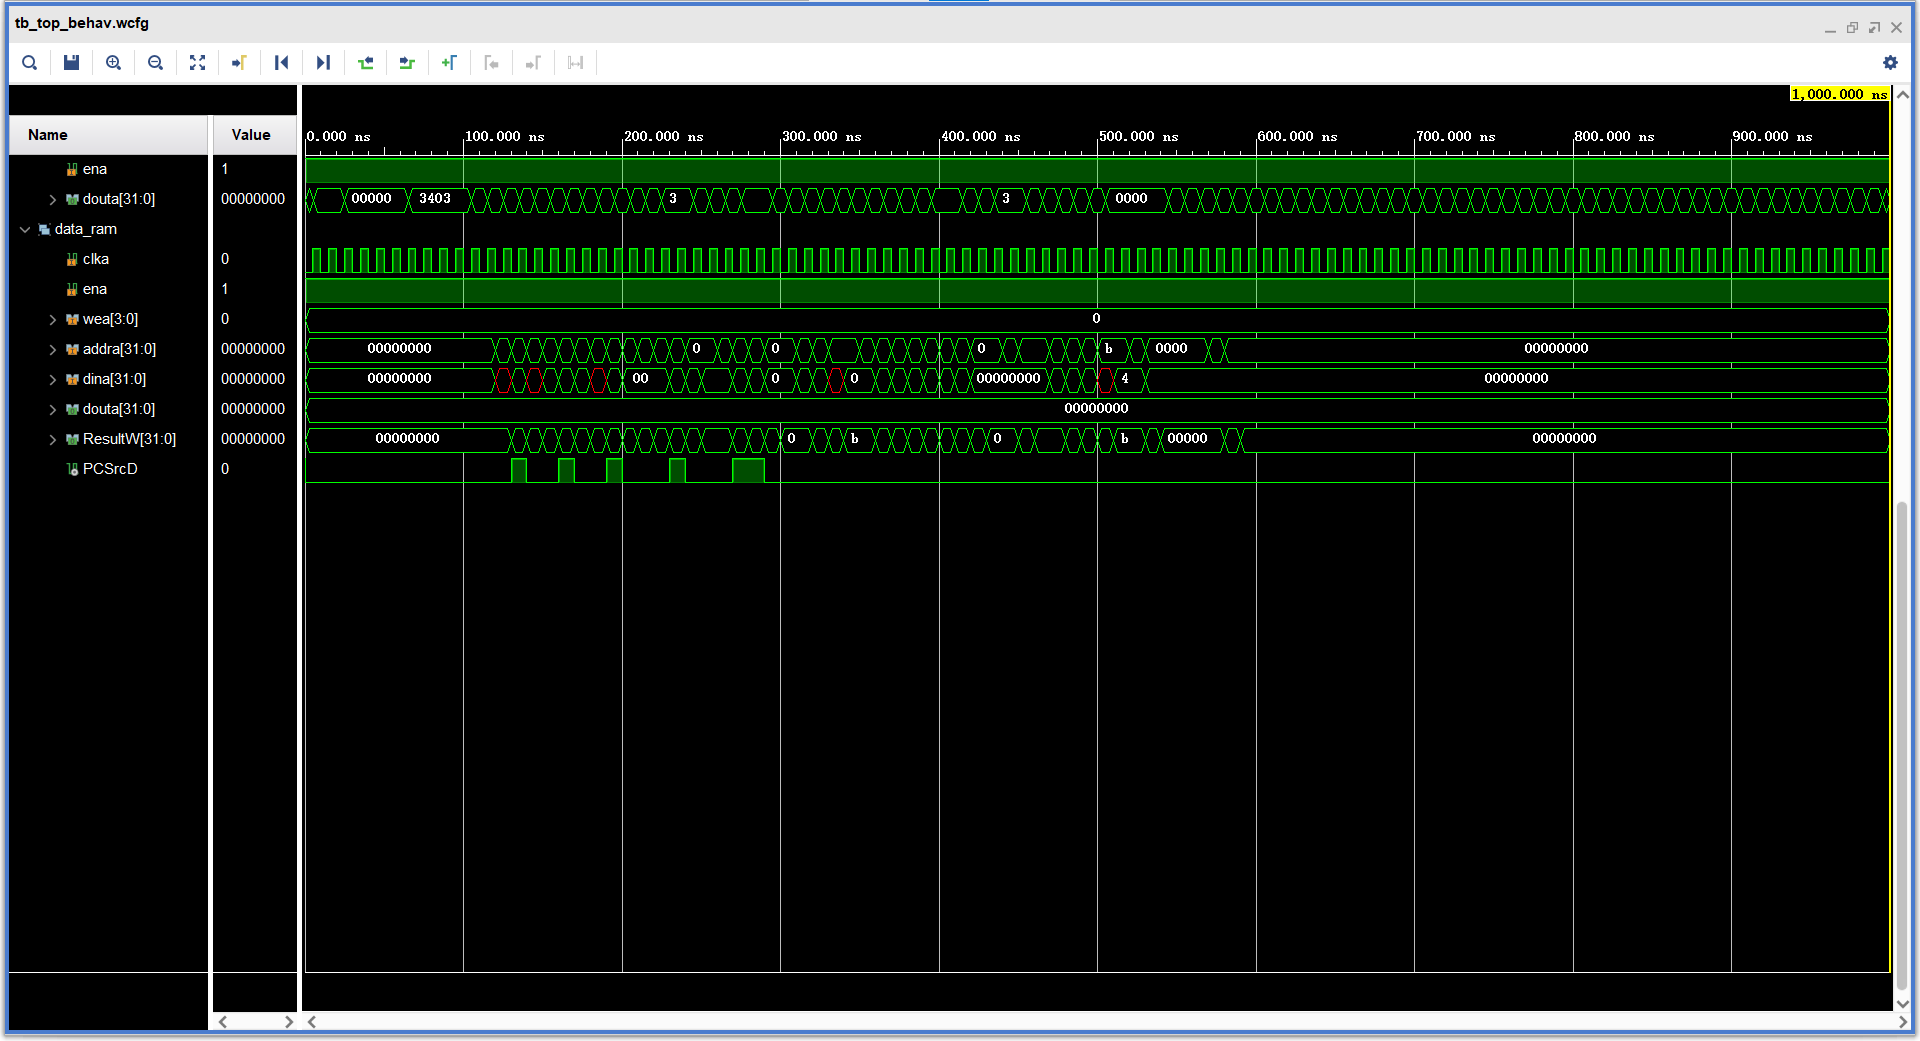
\includegraphics[width=\textwidth]{image/错误1-分析定位过程1.png}
    \caption{错误1-分析定位过程:查看 PCSrcD 信号}
    \label{fig:错误1-分析定位过程1}
\end{figure}

检查为 PCSrcD 赋值的各种条件,构造辅助信号查看其仿真波形图。

\begin{figure}[H]
    \centering
    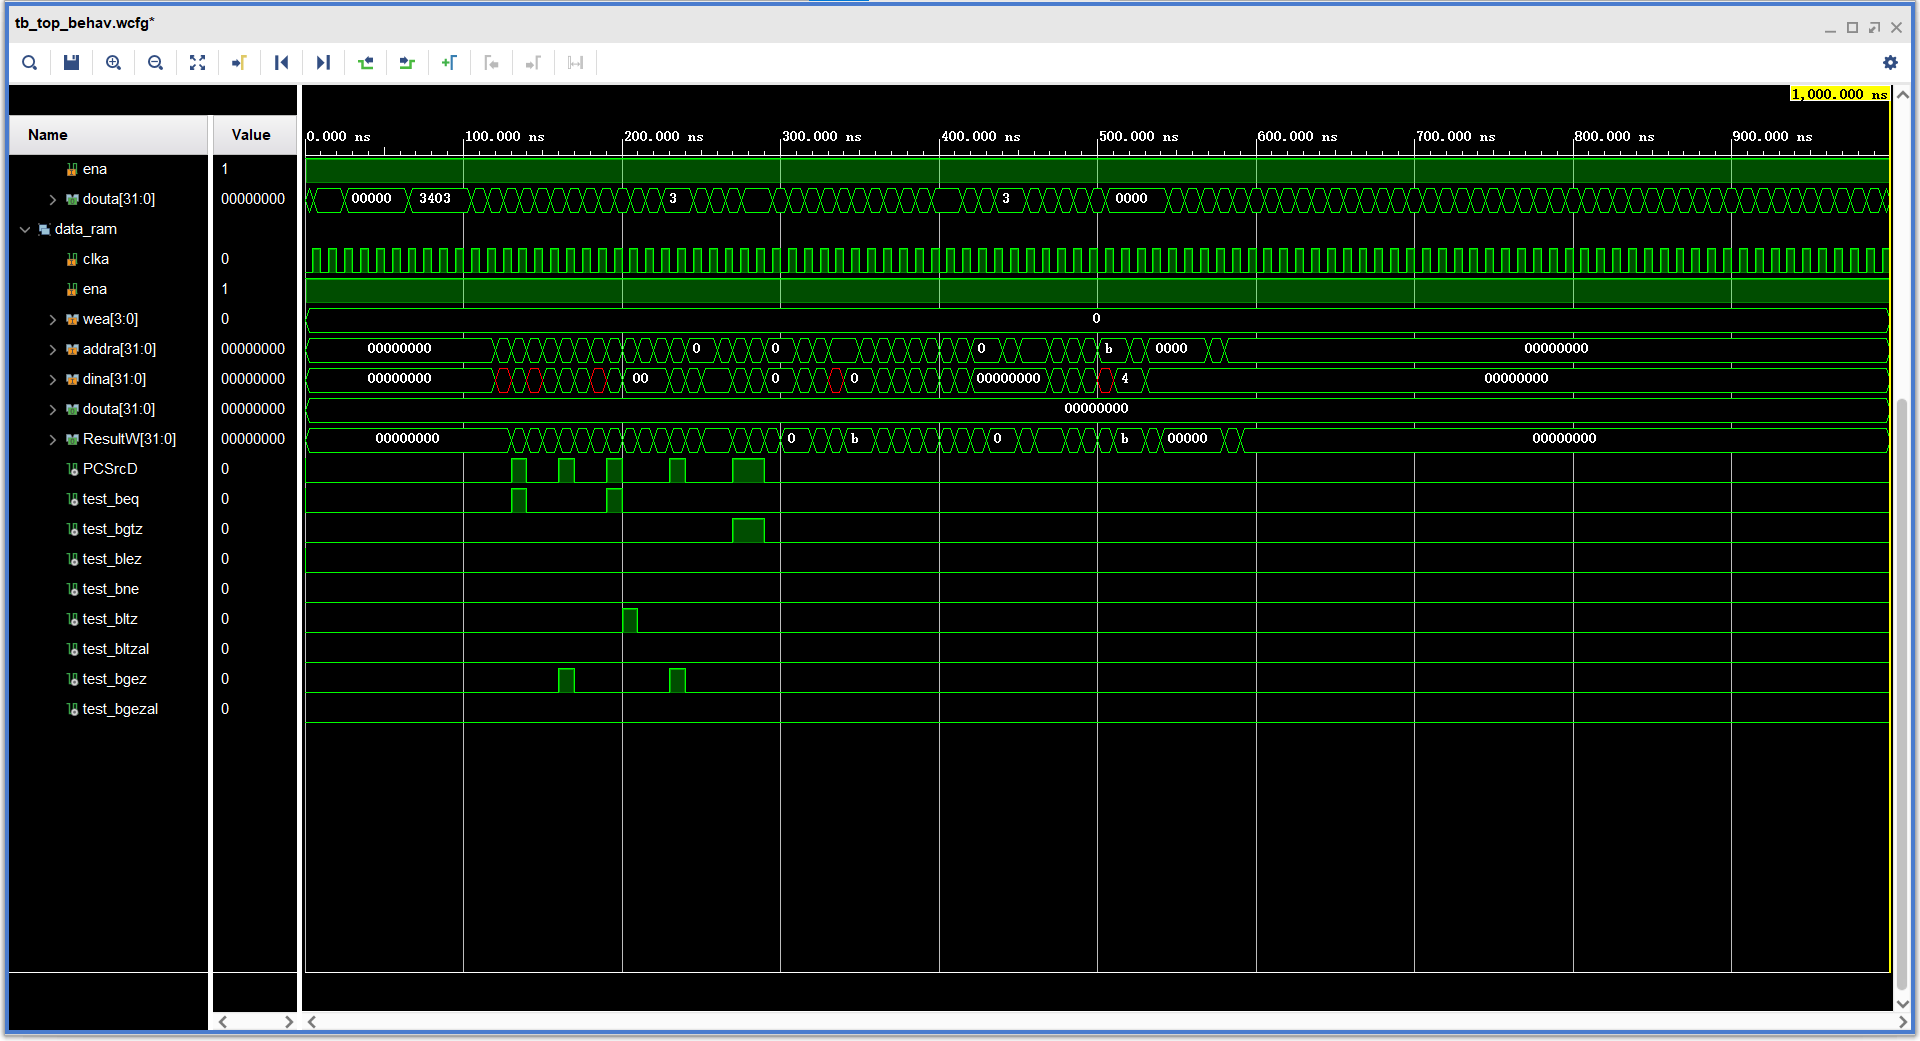
\includegraphics[width=\textwidth]{image/错误1-分析定位过程2.png}
    \caption{错误1-分析定位过程:查看 PCSrcD 信号}
    \label{fig:错误1-分析定位过程2}
\end{figure}

结合测试程序的汇编指令发现执行 BLTZ、BLTZAL、BGEZ、BGEZAL 指令时 PCSrcD 赋值错误。

在检查各指令对应的机器码 PCSrcD 赋值时发现这 4 条指令具有特殊的译码方式,在为 PCSrcD 赋值时译码错误。

    \item 错误原因

BLTZ、BLTZAL、BGEZ、BGEZAL 指令具有特殊的 Opcode 和译码方式,需要和其他分支指令进行区分。指令译码错误导致该错误发生。
    
    \item 修正效果

\begin{figure}[H]
    \centering
    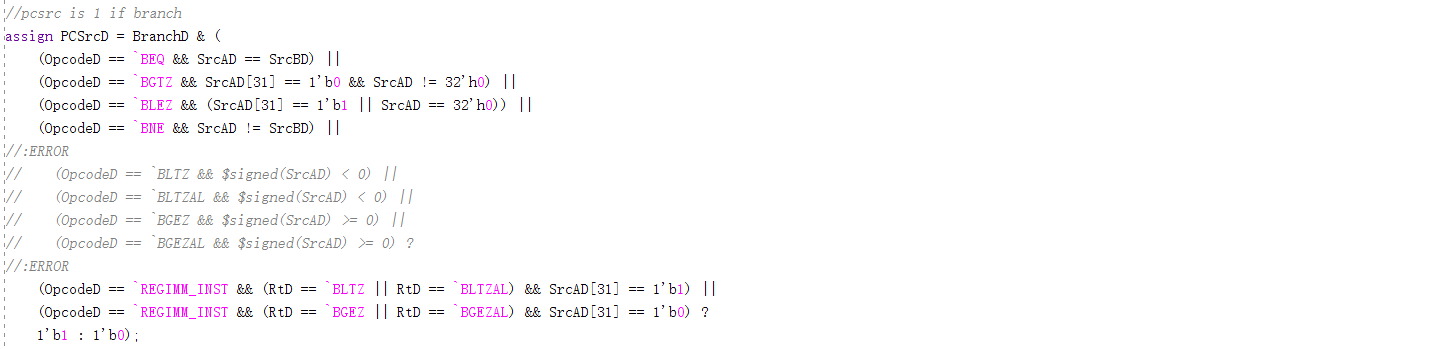
\includegraphics[width=\textwidth]{image/错误1-修正结果1.png}
    \caption{错误1-修正方式}
    \label{fig:错误1-修正结果1}
\end{figure}

改正后仿真波形图正确。

\begin{figure}[H]
    \centering
    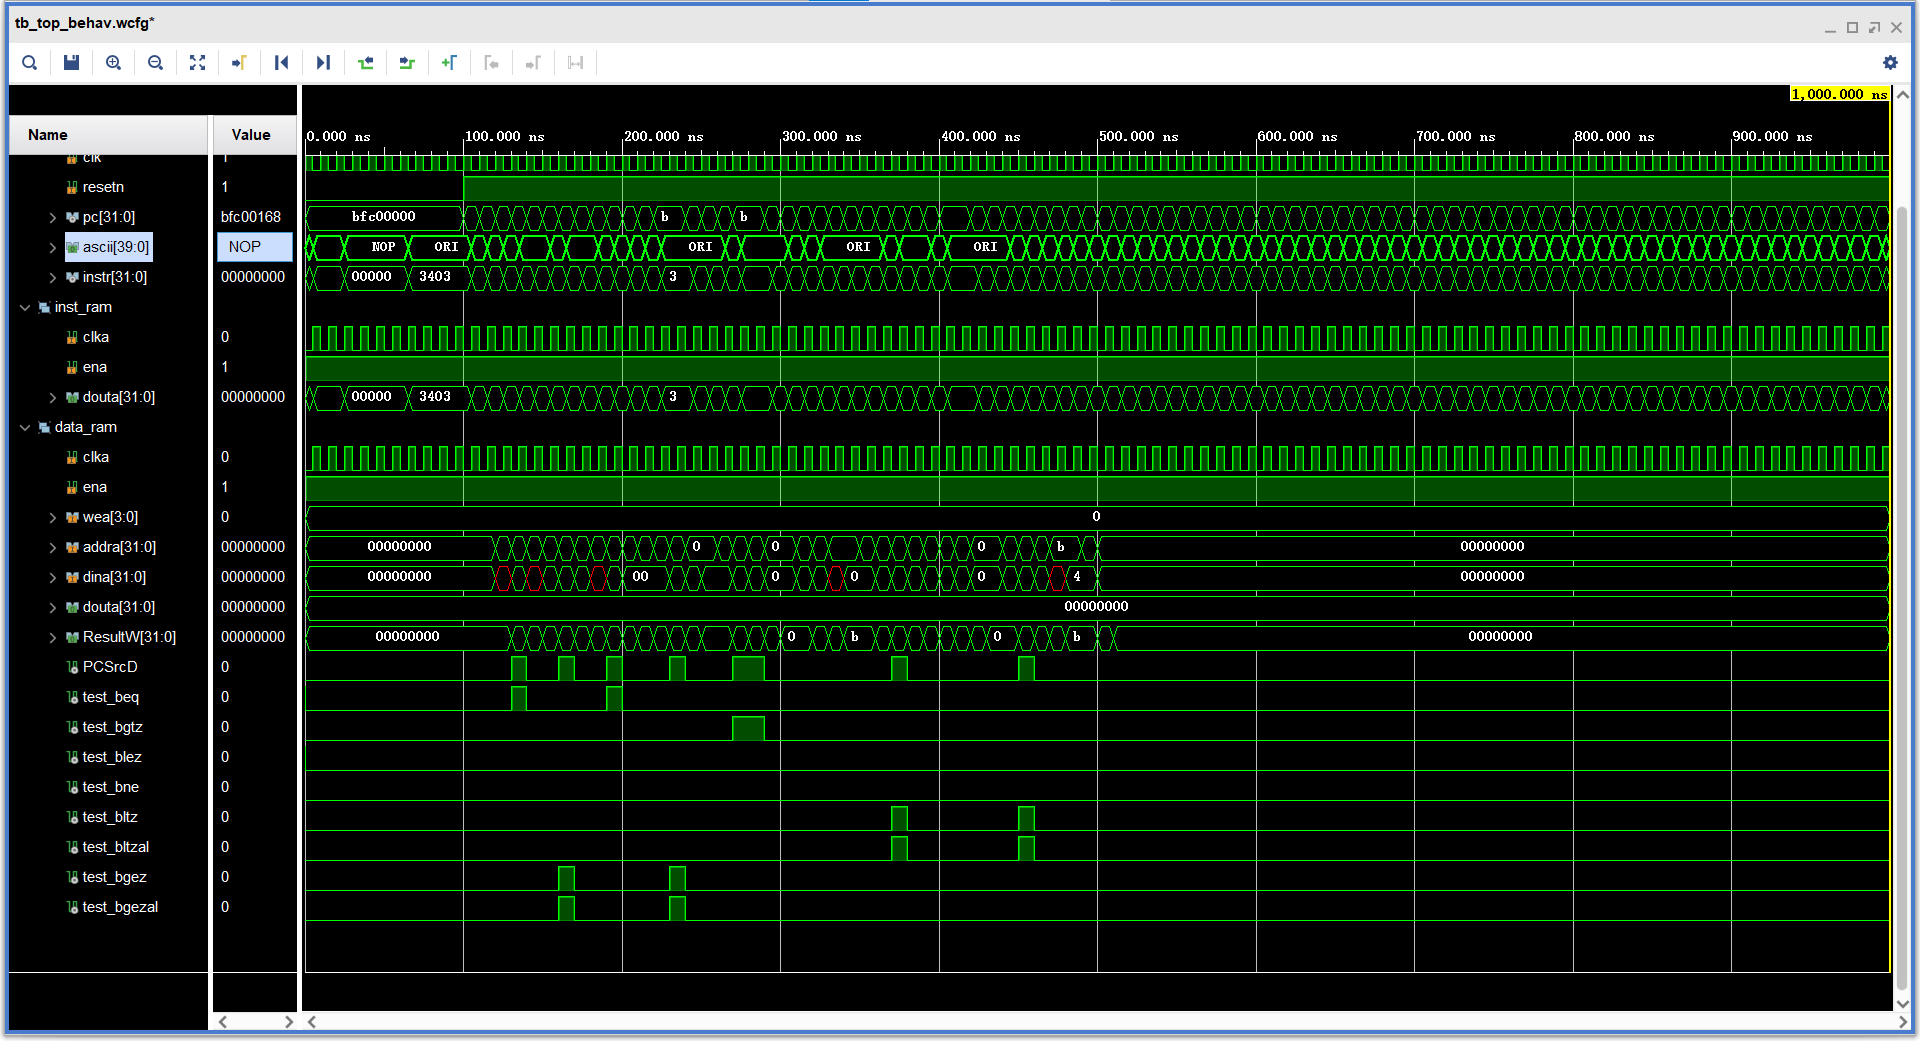
\includegraphics[width=\textwidth]{image/错误1-修正结果2.png}
    \caption{错误1-修正后的仿真波形图}
    \label{fig:错误1-修正结果1}
\end{figure}
    
    \item 归纳总结

需要特别注意特殊的指令格式。
    
\end{enumerate}

\subsubsection{错误2}

\begin{enumerate}[(1)]
    \item 错误现象

接入 SRAM 接口后,观察到运行后立刻出错。

\begin{figure}[H]
    \centering
    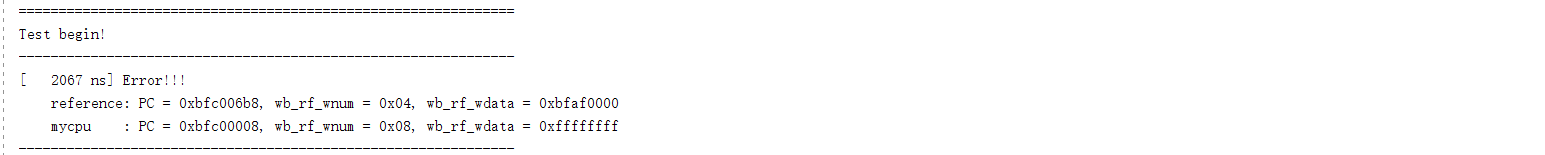
\includegraphics[width=\textwidth]{image/错误2-错误现象1.png}
    \caption{错误2-错误现象}
    \label{fig:错误2-错误现象1}
\end{figure}

\begin{figure}[H]
    \centering
    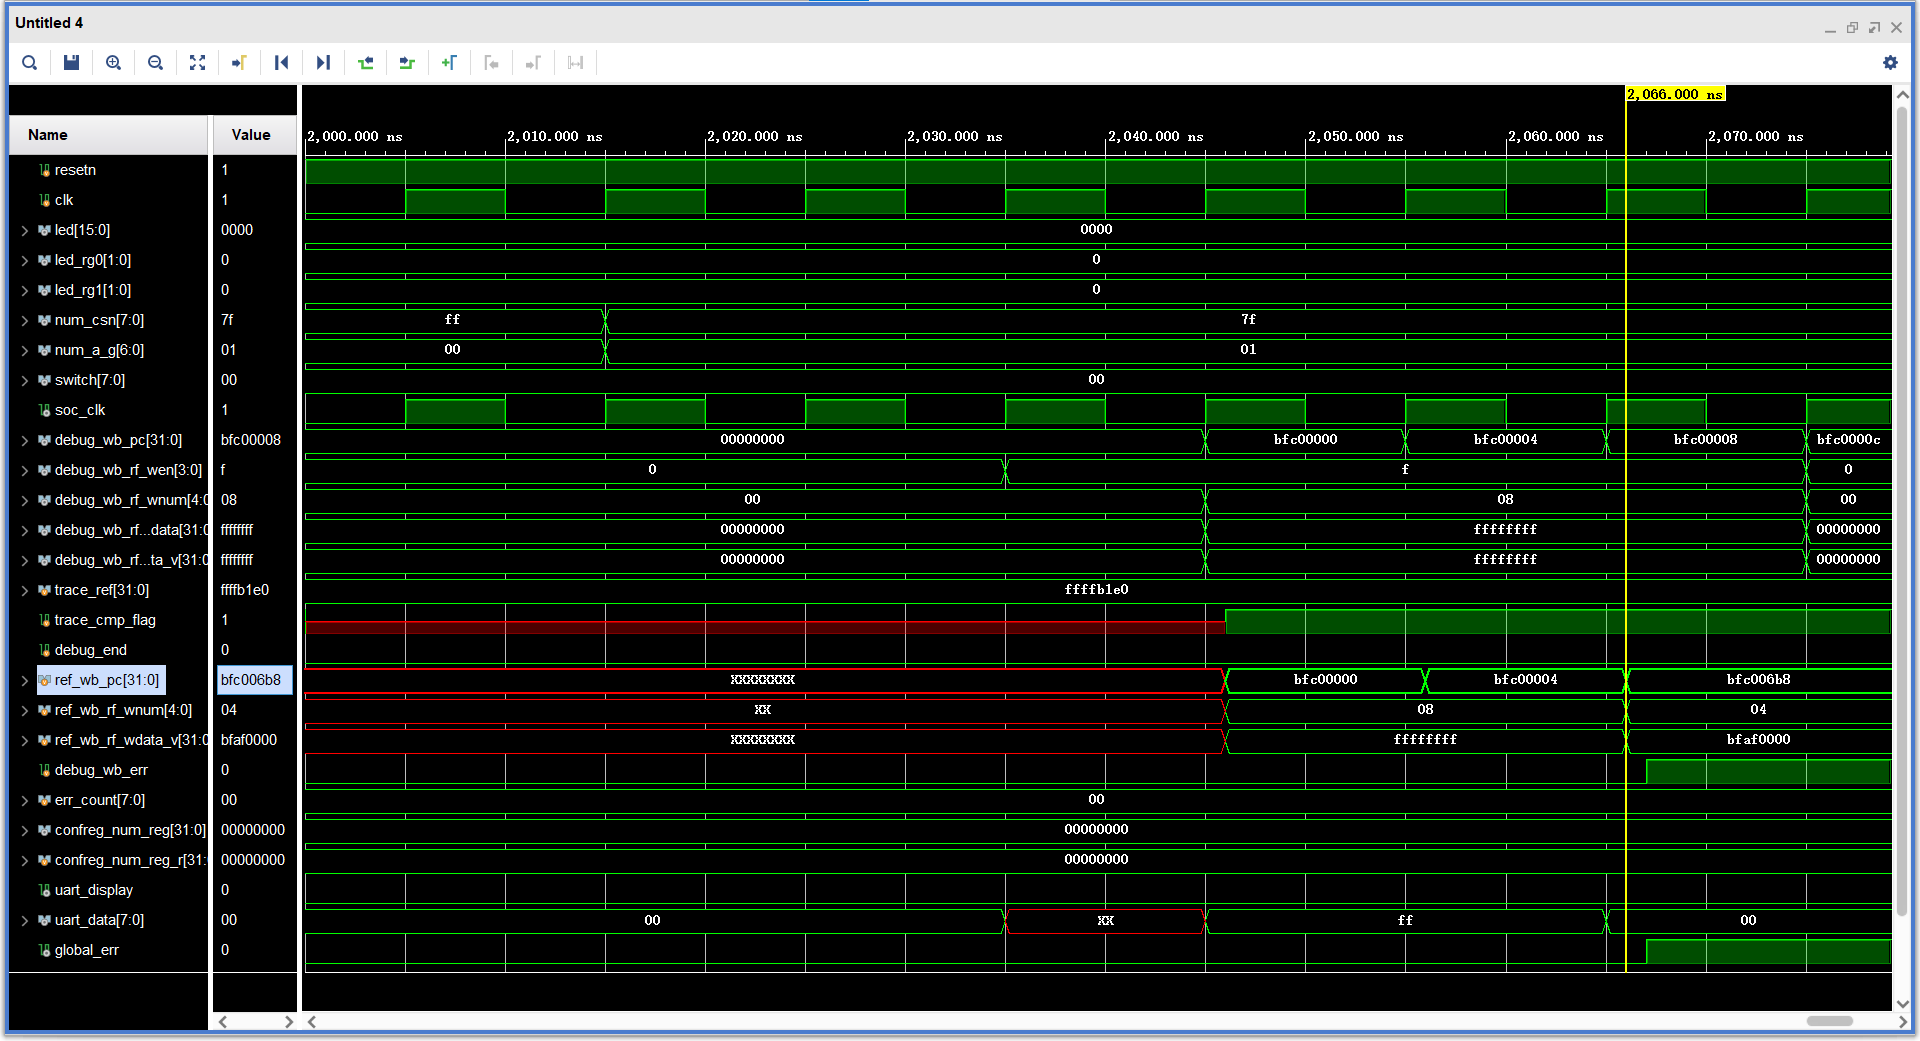
\includegraphics[width=\textwidth]{image/错误2-错误现象2.png}
    \caption{错误2-错误的仿真波形图 a}
    \label{fig:错误2-错误现象2}
\end{figure}

接入 SRAM 接口后,观察到 PC 始终为 0。

\begin{figure}[H]
    \centering
    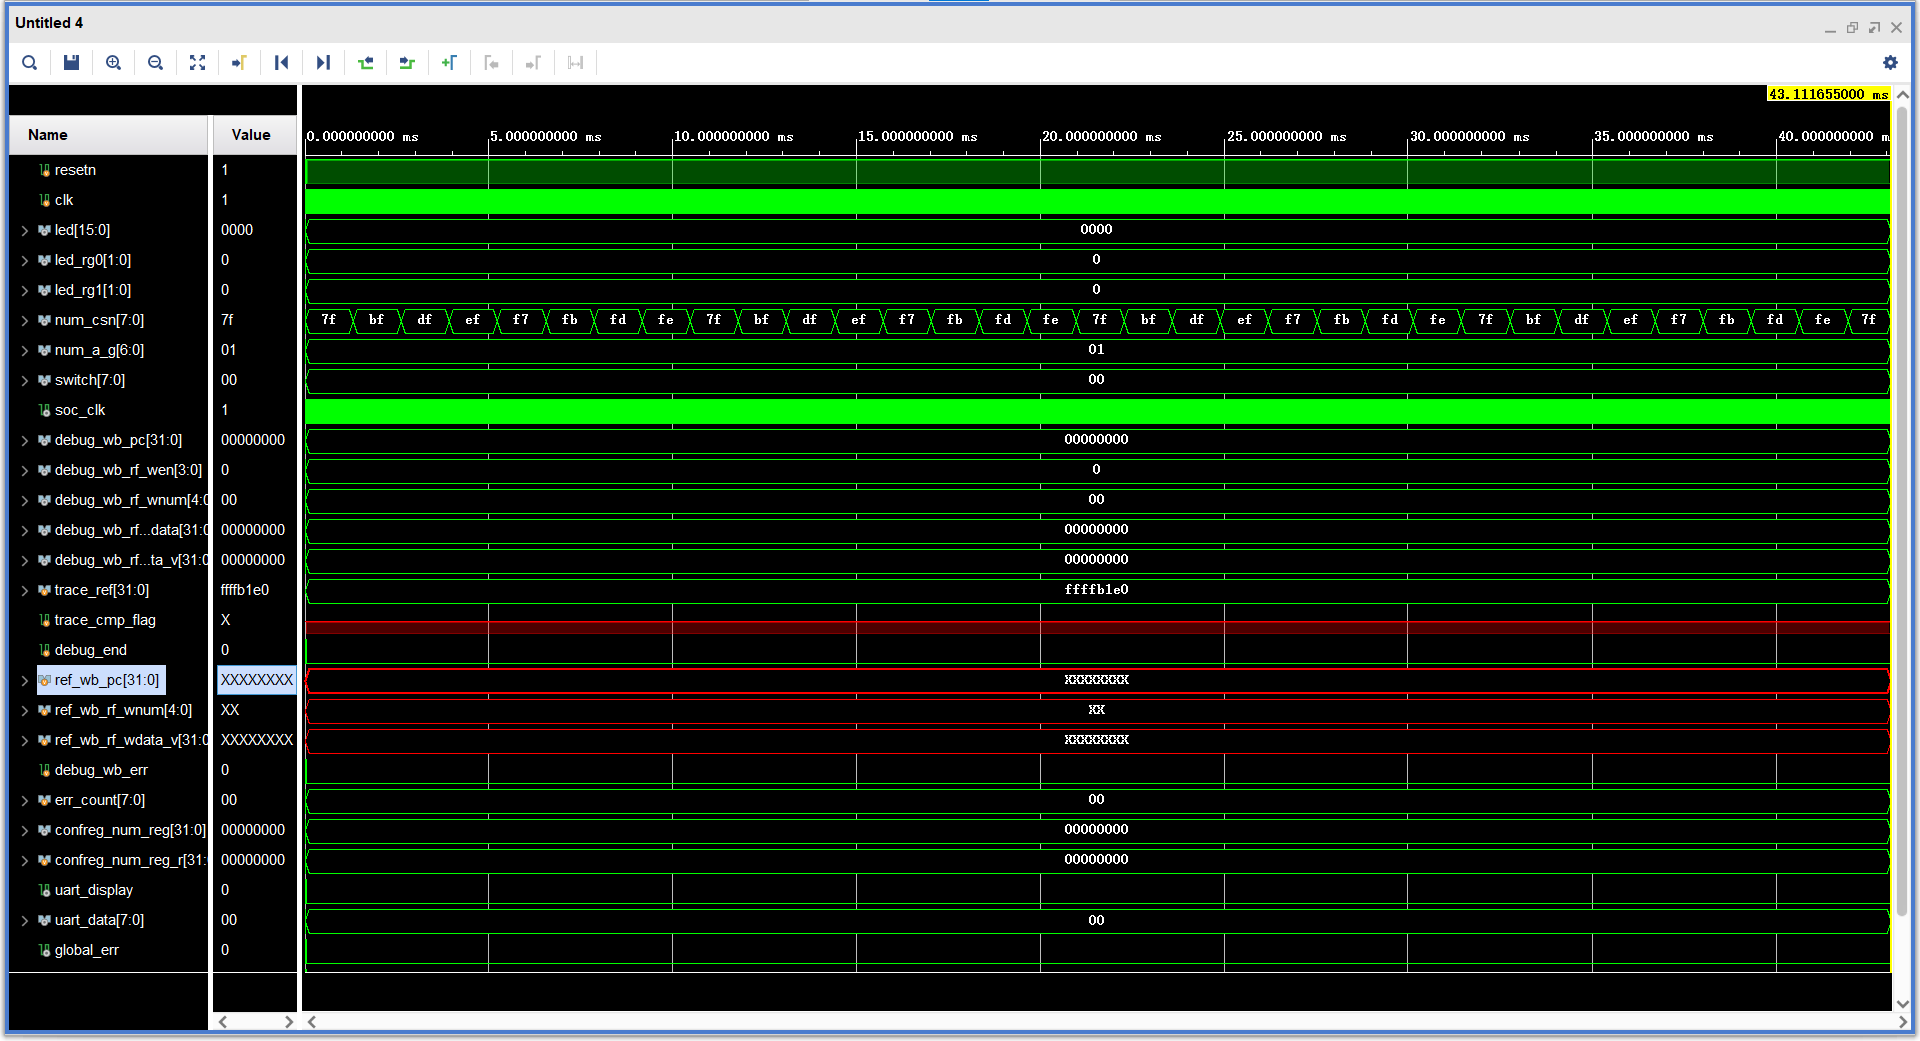
\includegraphics[width=\textwidth]{image/错误2-错误现象3.png}
    \caption{错误2-错误的仿真波形图 b}
    \label{fig:错误2-错误现象3}
\end{figure}

    \item 分析定位过程

由于已经通过按指令分类的功能测试,推测错误原因为连接 SRAM 接口错误。观察到仿真波形图中 resetn 为高电平有效,又仔细对比实验文档内容,发现 clock 和 resetn 信号未取反。

    \item 错误原因

连接 SRAM 接口的 clock 和 resetn 信号未取反。
    
    \item 修正效果

按照实验文档中的说明设置 clock 和 resetn 信号。

\begin{figure}[H]
    \centering
    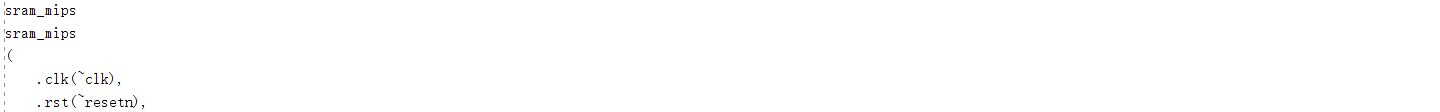
\includegraphics[width=\textwidth]{image/错误2-修正效果1.png}
    \caption{错误2-修正方式}
    \label{fig:错误2-修正效果1}
\end{figure}

各信号严格按照实验文档指导取值后解决此错误,SRAM 功能测试能够运行。
    
    \item 归纳总结

    仔细阅读实验文档。
    
\end{enumerate}

\subsubsection{错误3}

\begin{enumerate}[(1)]
    \item 错误现象

在 SRAM 功能测试的第 65 个测试点(syscall 异常测试)触发 syscall 异常后立刻出错;PC 和 wb\_rf\_wnum 均正确,而 wb\_rf\_wdata 错误。

\begin{figure}[H]
    \centering
    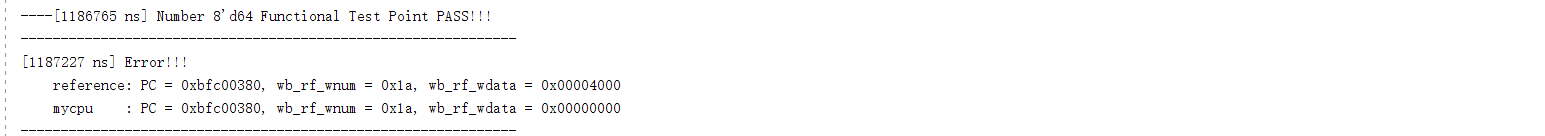
\includegraphics[width=\textwidth]{image/错误3-错误现象1.png}
    \caption{错误3-错误现象}
    \label{fig:错误3-错误现象1}
\end{figure}

    \item 分析定位过程

地址 0xbfc00380 恰好是异常处理程序的入口地址。查看测试程序的汇编指令,该地址对应汇编指令为

\begin{lstlisting}
bfc00380:	0000d010 	mfhi	k0
\end{lstlisting}

推测错误原因为 HILO 寄存器相关错误。

将 HILO 寄存器相关信号 HiLoIE、HiLoOE、HiLoIM、HiLoOM 添加到仿真波形图中,观察到信号 HiLoIE、HiLoOE、HiLoIM 均在异常发生时被刷新,而 HiLoOM 不变。

\begin{figure}[H]
    \centering
    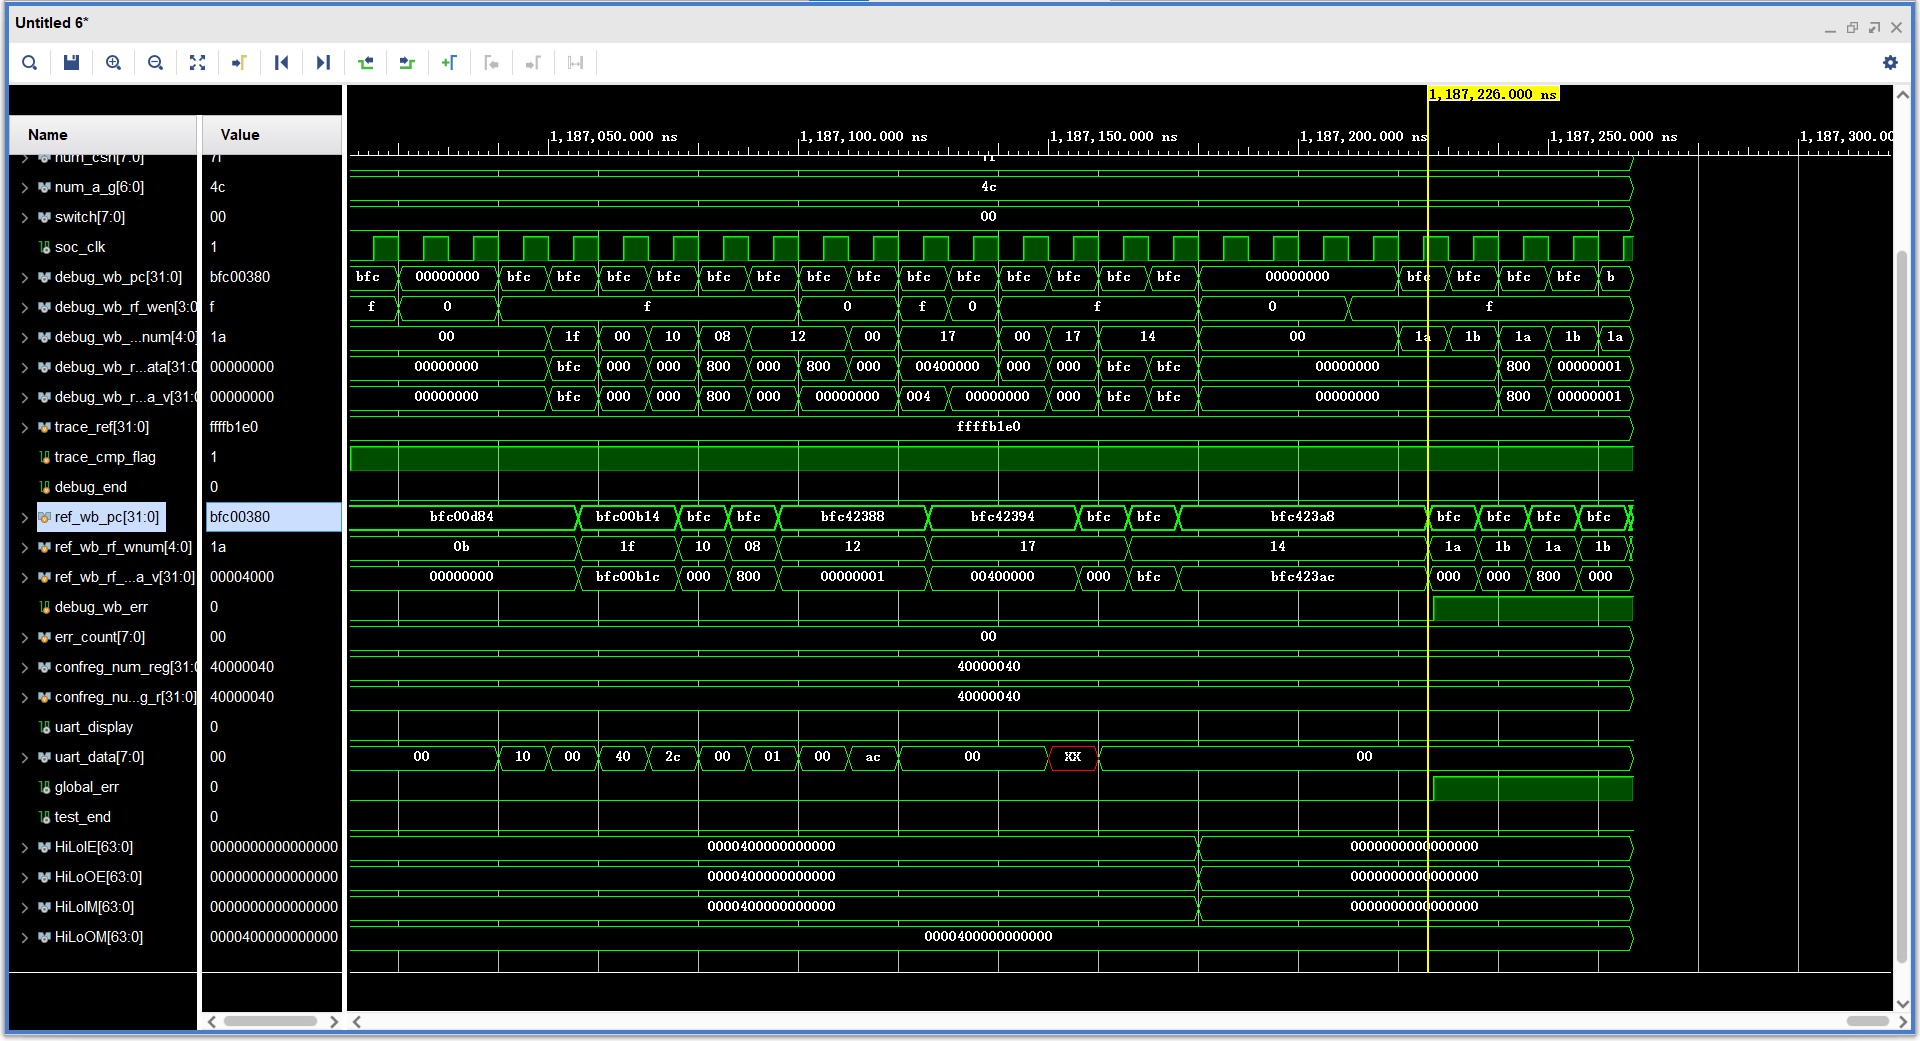
\includegraphics[width=\textwidth]{image/错误3-分析定位过程1.png}
    \caption{错误3-HILO 寄存器相关信号的仿真波形图}
    \label{fig:错误3-分析定位过程1}
\end{figure}

观察设计的数据通路中相关逻辑,HiLoOM 为 HILO 寄存器输出值。

\begin{figure}[H]
    \centering
    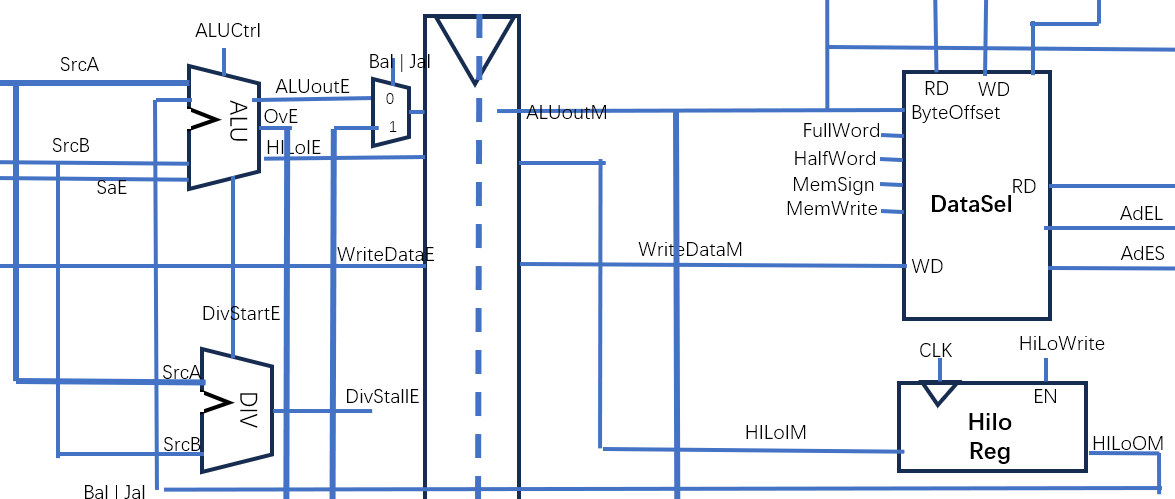
\includegraphics[width=\textwidth]{image/错误3-分析定位过程2.png}
    \caption{错误3-HILO 寄存器相关数据通路图}
    \label{fig:错误3-分析定位过程2}
\end{figure}

因此 HILO 寄存器内数据并无错误。结合数据通路图继续检查相关连线,发现 HiLoOE 的连线错误,进而使设计中 ALU 和 HILO 寄存器之间形成的环路 ALU -> HiLoIE -> HiLoIM -> HiLoReg -> HiLoOM -> ALU 被错误地连接为 ALU -> HiLoIE -> HiLoIM -> HiLoReg 和 ALU -> HiLoIE -> HiLoIM -> HiLoOE -> ALU。

\begin{figure}[H]
    \centering
    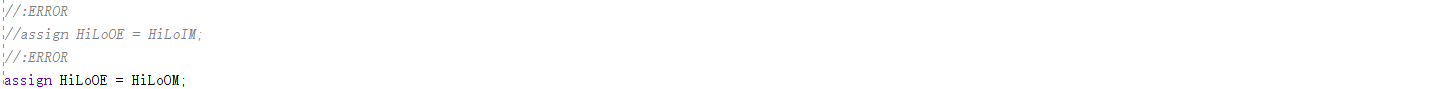
\includegraphics[width=\textwidth]{image/错误3-分析定位过程3.png}
    \caption{错误3-HILO 连线修正}
    \label{fig:错误3-分析定位过程3}
\end{figure}

    \item 错误原因

HILO 寄存器与 ALU 之间的连线与设计的数据通路不同导致错误。

在流水线未被刷新时,HiLoIM 的值将与 HiLoIE 的值相等,而流水线 EX\_MEM 间接地起到了 HILO 寄存器的作用,因此即使未实际连接到 HILO 寄存器,相关指令仍然能够正常执行。这也是在按功能分类的功能测试中无法发现这个错误的原因。

当异常发生时,流水线被刷新,这相当于将 HILO 寄存器(EX\_MEM 中的 HiLoIE)清空。由于没有其他值输入 HiLoIM,因此流水线刷新后 HiLoIE、HiLoOE、HiLoIM 将始终为 0。而由于 HiLoOM 被保存在实际的 HILO 寄存器中,所以直到下一次执行 MTHI 或 MTLO 指令时其值不会改变。从流水线刷新后到下一次执行 MTHI 或 MTLO 指令前,所有 MFHI 或 MFLO 指令的执行将向寄存器 rd 中写入 0。
    
    \item 修正效果

按图\ref{fig:错误3-分析定位过程3}所示方式修正后,顺利解决此错误,通过了 syscall 等若干涉及异常处理的测试点。
    
\end{enumerate}


\subsubsection{错误4}

\begin{enumerate}[(1)]
    \item 错误现象

在 SRAM 功能测试的第 73 个测试点(SW 指令触发 AdES 异常测试)中,位于地址 0xbfc0d044 的指令

\begin{lstlisting}
bfc0d044:	8c824188 	lw	v0,16776(a0)
\end{lstlisting}

加载的数据错误。

\begin{figure}[H]
    \centering
    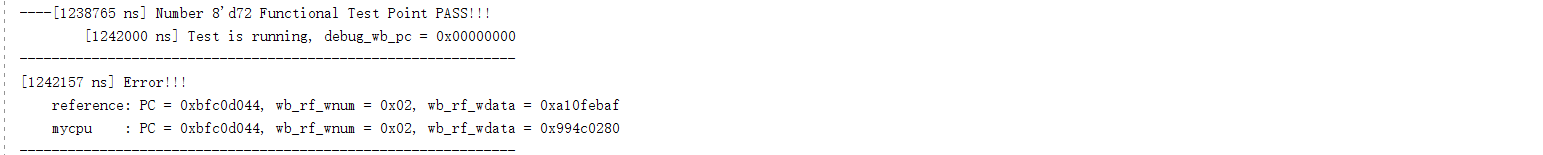
\includegraphics[width=\textwidth]{image/错误4-错误现象1.png}
    \caption{错误4-错误现象}
    \label{fig:错误4-错误现象1}
\end{figure}

\begin{figure}[H]
    \centering
    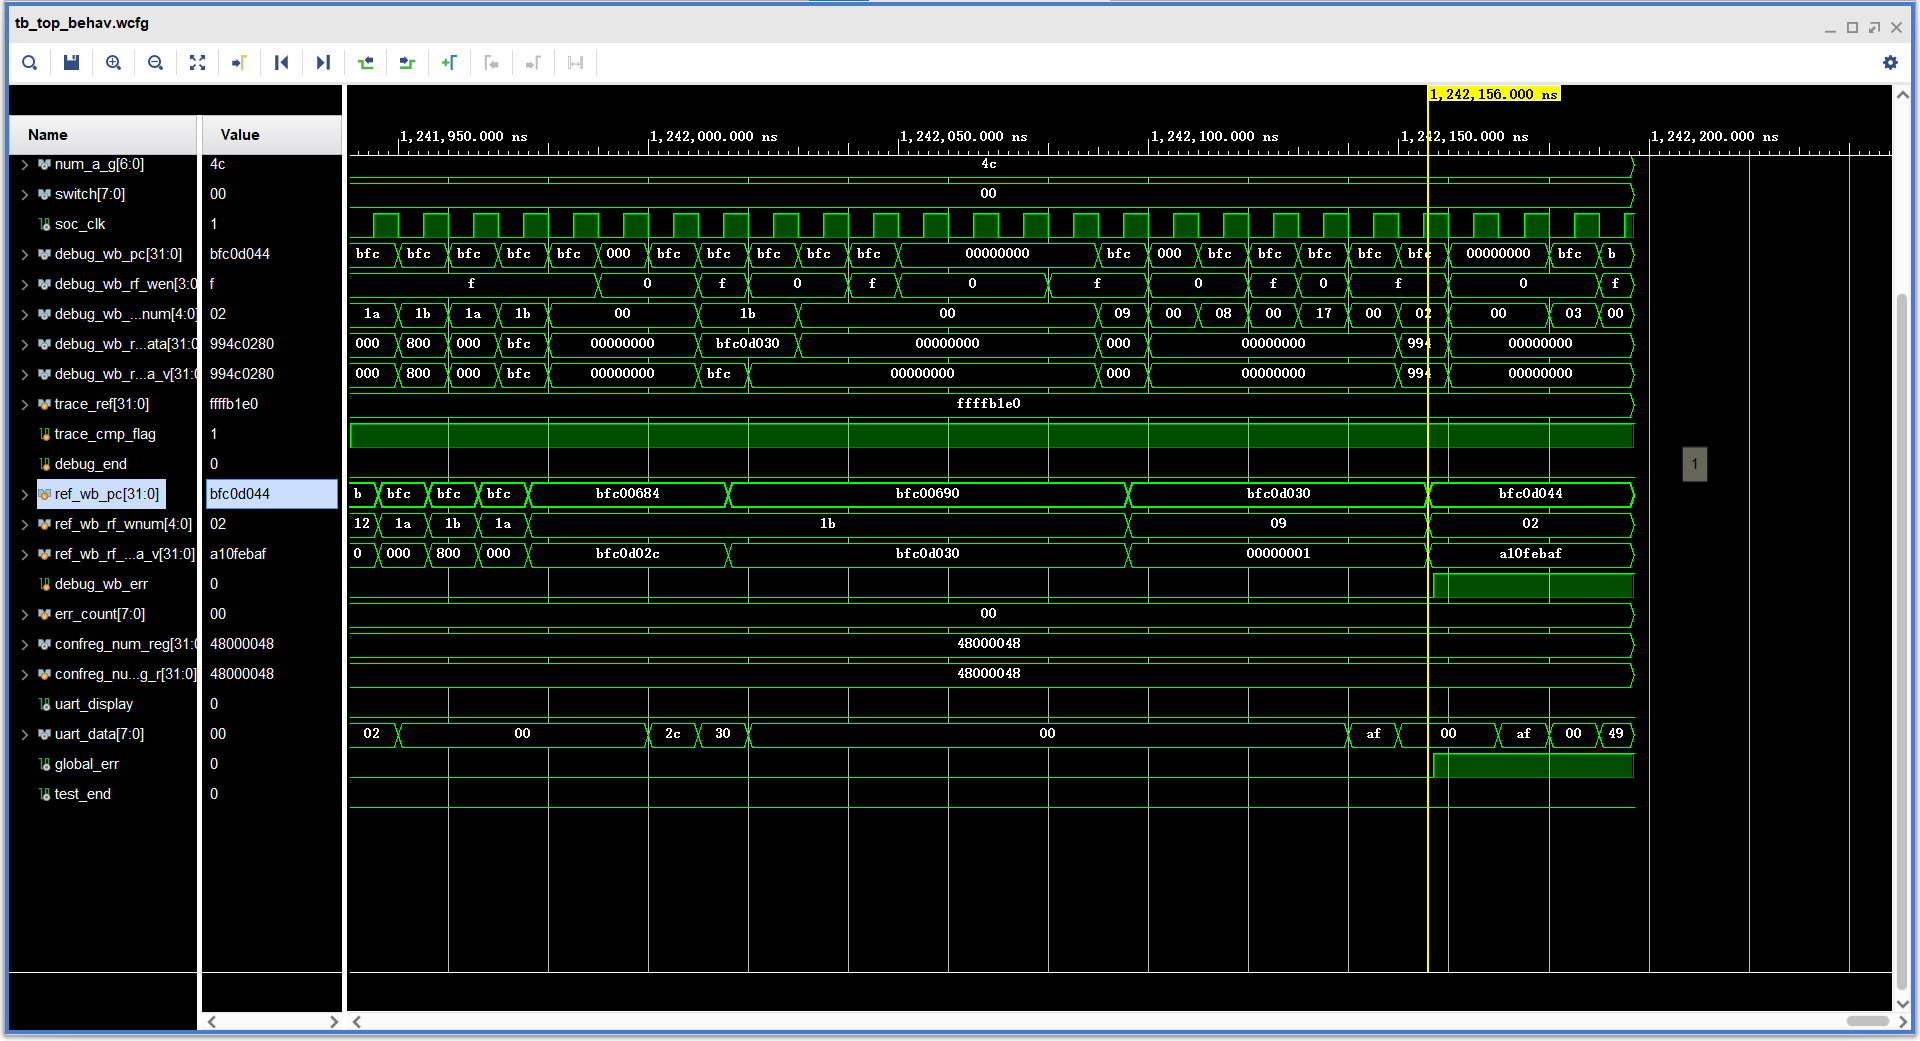
\includegraphics[width=\textwidth]{image/错误4-错误现象2.png}
    \caption{错误4-错误的仿真波形图}
    \label{fig:错误4-错误现象2}
\end{figure}

    \item 分析定位过程

查看测试程序的汇编指令。执行出错的指令将位于地址 16776(a0) 的数据读入寄存器。找到最近一次将数据写入该地址的指令为位于地址 0xbfc0d018 的指令

\begin{lstlisting}
bfc0d018:	ac824188 	sw	v0,16776(a0)
\end{lstlisting}

该指令使用的寄存器 v0 和 a0 的值在此前通过指令设置:

\begin{lstlisting}
...
bfc0cff4:	3c02a10f 	lui	v0,0xa10f
bfc0cff8:	3442ebaf 	ori	v0,v0,0xebaf
...
bfc0d004:	3c04800d 	lui	a0,0x800d
bfc0d008:	34848850 	ori	a0,a0,0x8850
...
\end{lstlisting}

计算存入寄存器 v0 和 a0 中的值可以发现 地址 16776(a0) 是 4 的倍数,此时将不产生 AdES 异常。将 ExceptTypeM 添加到仿真波形图,向前找到地址 0xbfc0d018,观察到执行该指令时 ExceptTypeM 始终为 0。这说明错误的原因不在这里。

观察仿真波形图发现在执行位于地址 0xbfc0d02c 的指令

\begin{lstlisting}
bfc0d02c:	ac85418b 	sw	a1,16779(a0)
\end{lstlisting}

时产生 AdES 异常。经过仔细观察发现,地址 16779(a0) 与 16776(a0) 仅相差 3 字节。猜想错误的原因是这条指令的执行使内存中的数据改变。

将控制写内存的信号 DataEn 添加到仿真波形图中,观察到最后一次 DataEn 信号不为 0 时恰好执行这条指令。这证实了上面的猜想。对应的解决方案是在触发 AdES 异常时将 DataEn 信号置为 0。

\begin{figure}[H]
    \centering
    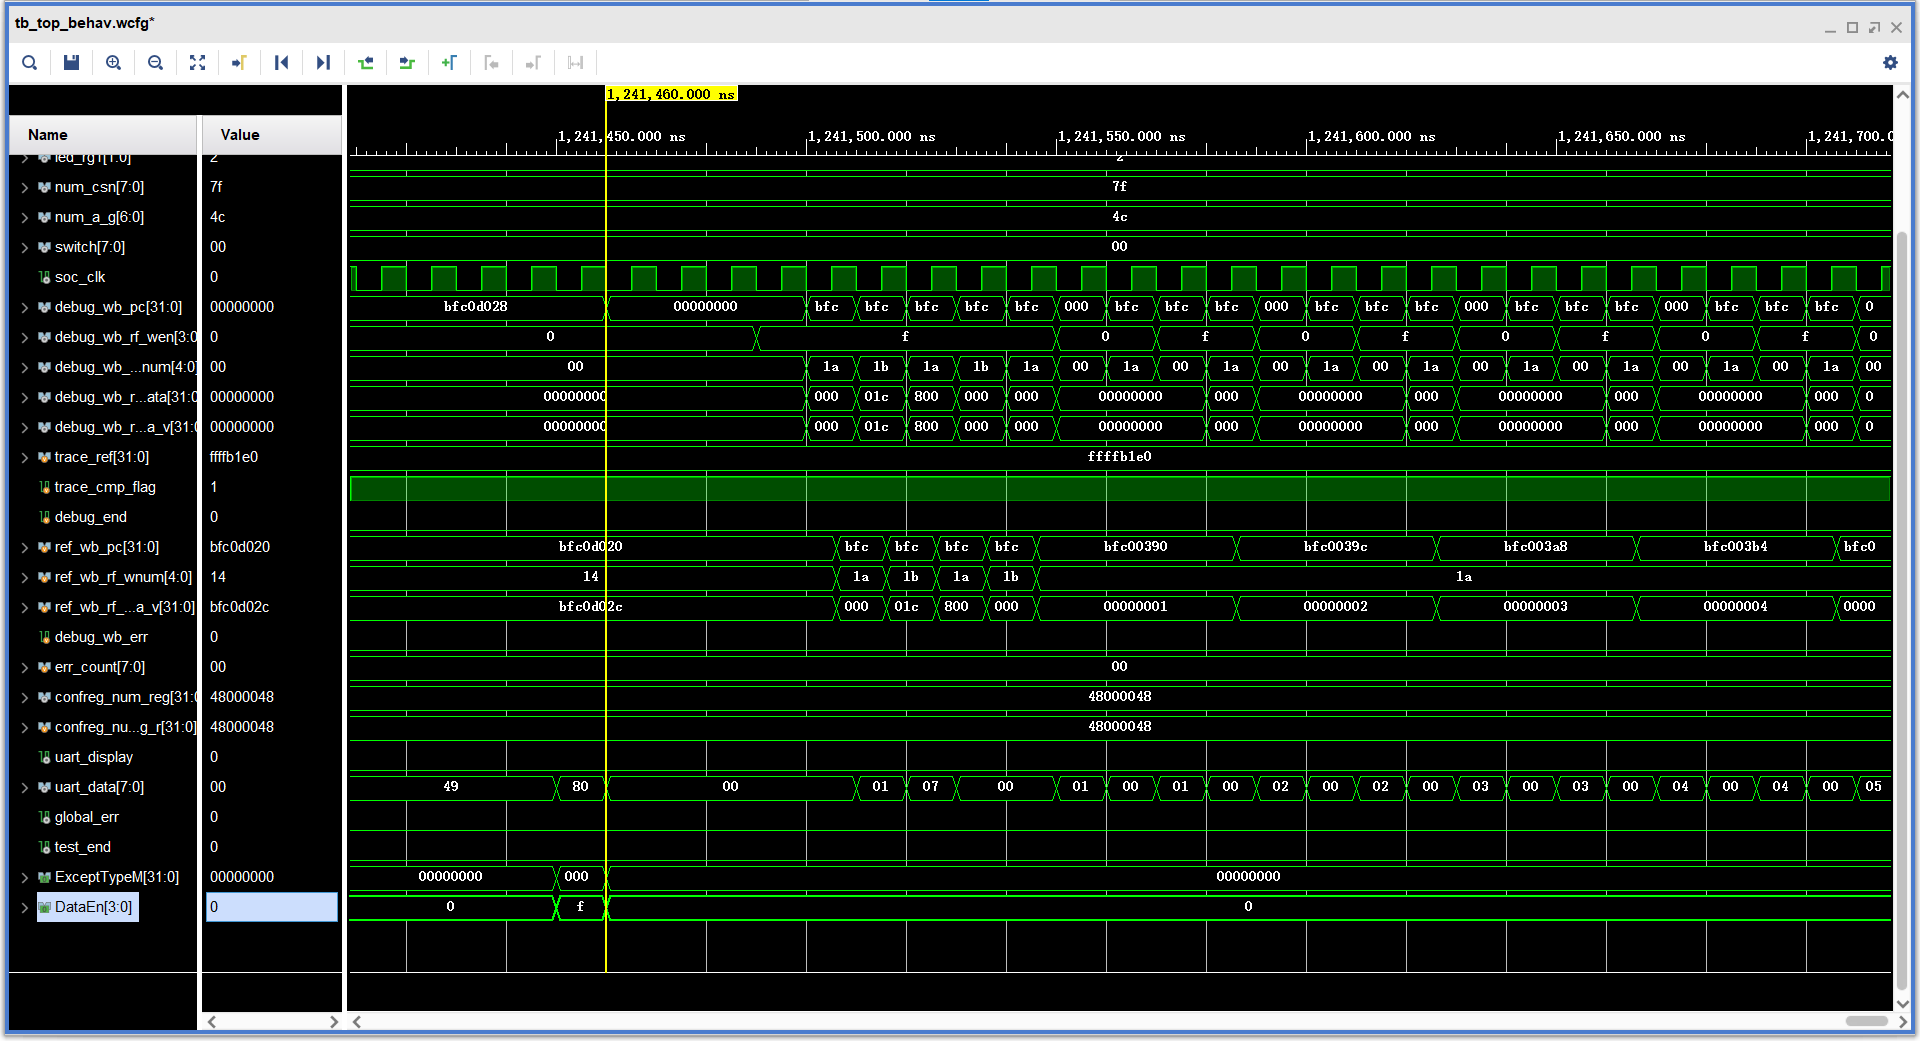
\includegraphics[width=\textwidth]{image/错误4-分析定位过程1.png}
    \caption{错误4-DataEn 信号的值说明错误的原因是发生 AdES 异常时将错误的数据写入内存}
    \label{fig:错误4-分析定位过程1}
\end{figure}

    \item 错误原因

触发 AdES 异常时仍然能够向数据存储器中写入数据导致数据被改变造成。
    
    \item 修正效果

进行图\ref{fig:错误4-修正效果1}所示修改后解决了该错误,并通过了第 65 个测试点。

\begin{figure}[H]
    \centering
    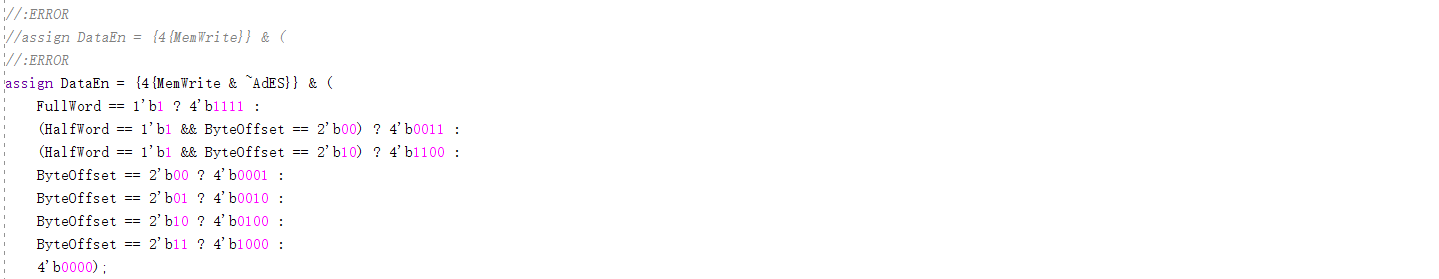
\includegraphics[width=\textwidth]{image/错误4-修正效果1.png}
    \caption{错误4-修正方式 a}
    \label{fig:错误4-修正效果1}
\end{figure}

参考 2019 年硬件综合设计讲解视频,可以得出第二种可行的办法,即在发生异常时将数据存储器的使能信号置为 0。

\begin{figure}[H]
    \centering
    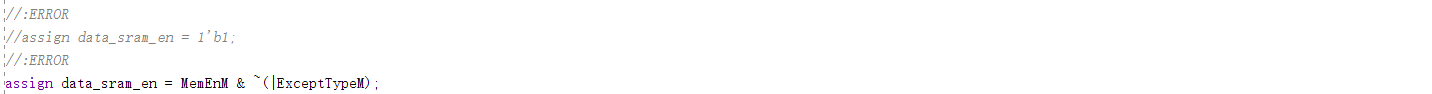
\includegraphics[width=\textwidth]{image/错误4-修正效果2.png}
    \caption{错误4-修正方式 b}
    \label{fig:错误4-修正效果2}
\end{figure}

两种修正方案具有相同的效果。这是因为只有在写内存时才可能修改其中的数据,并且写内存时可能发生的异常只有 AdES 异常。

\end{enumerate}


\subsubsection{错误5}

\begin{enumerate}[(1)]
    \item 错误现象

接入 AXI 接口后,观察到运行后立刻出错。

\begin{figure}[H]
    \centering
    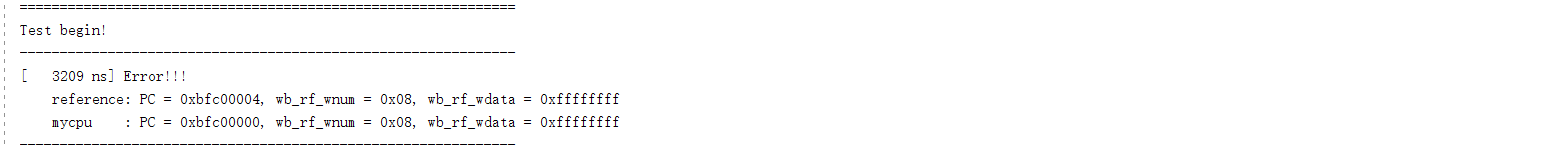
\includegraphics[width=\textwidth]{image/错误5-错误现象1.png}
    \caption{错误5-错误现象}
    \label{fig:错误5-错误现象1}
\end{figure}

\begin{figure}[H]
    \centering
    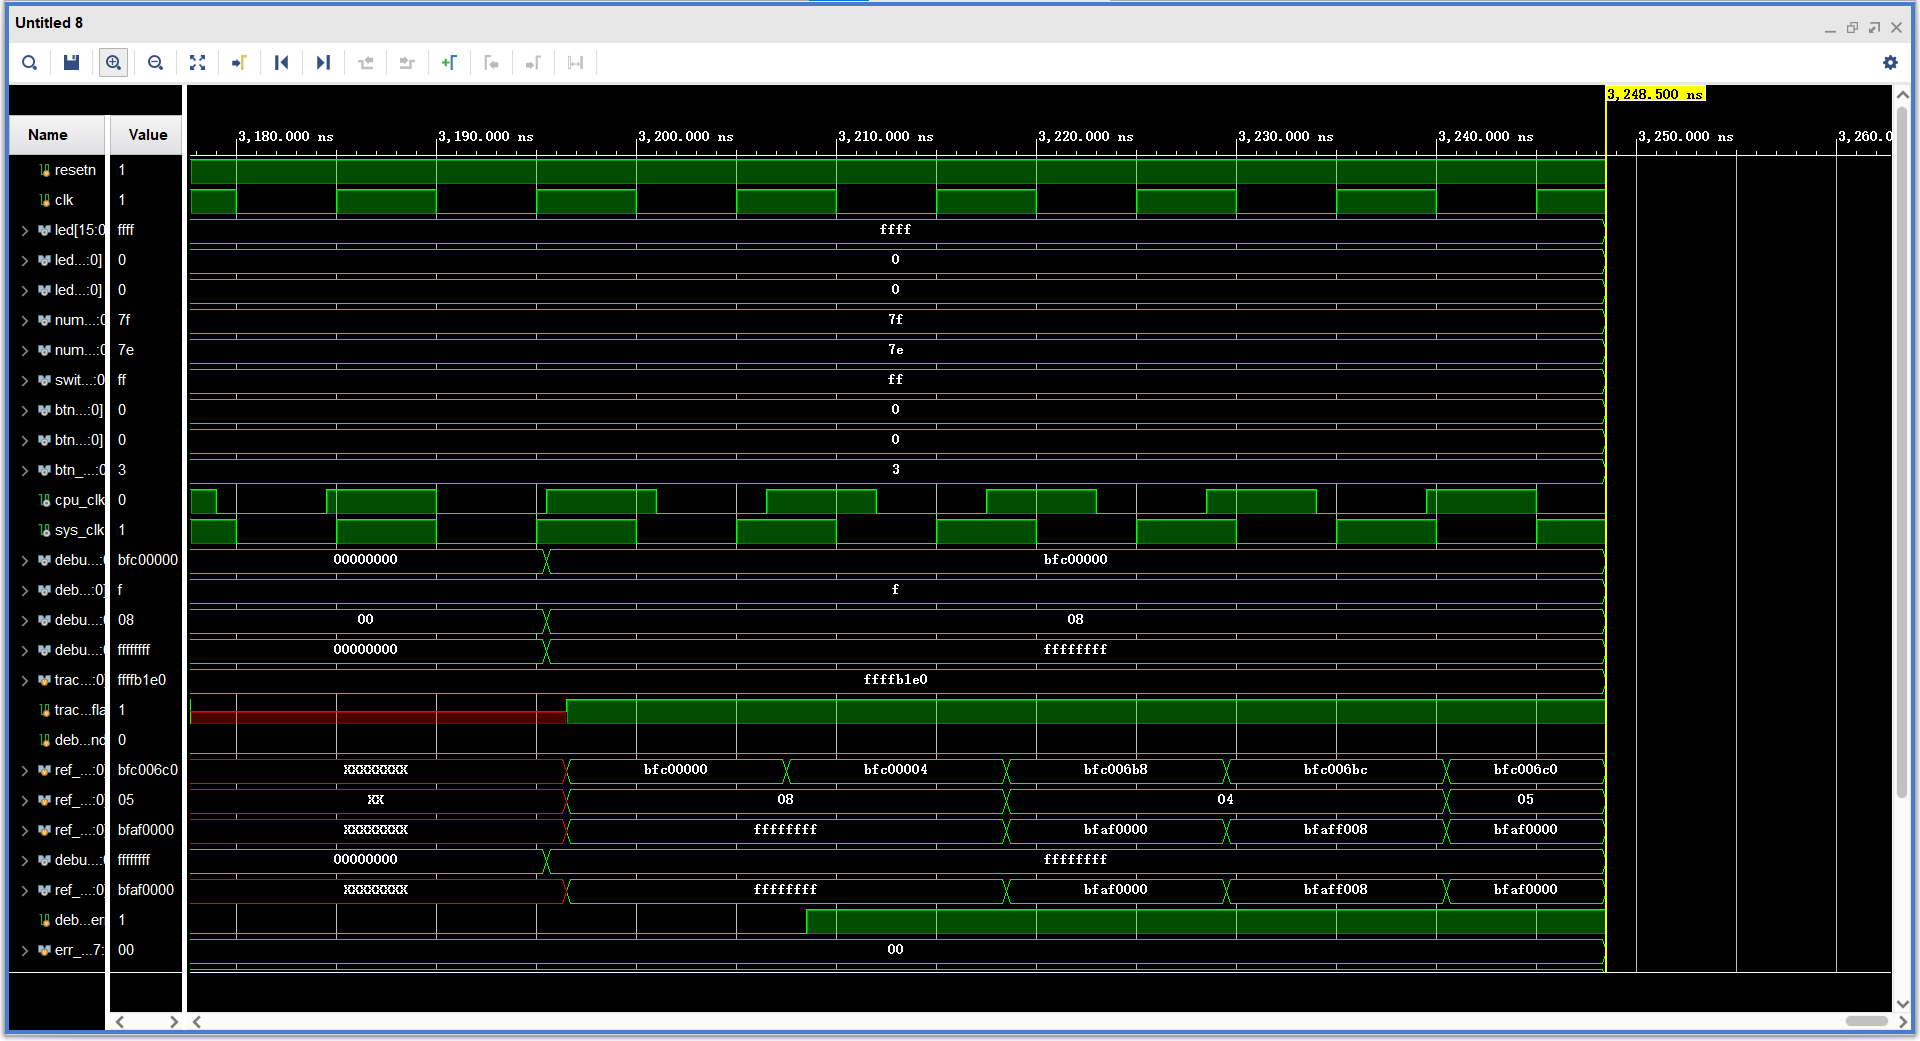
\includegraphics[width=\textwidth]{image/错误5-错误现象2.png}
    \caption{错误5-错误的仿真波形图}
    \label{fig:错误5-错误现象2}
\end{figure}

    \item 分析定位过程

观察仿真波形图。与 SRAM 接口中访问内存不额外占用时钟周期的实现相比,AXI 接口的实现在访问内存时占用多个时钟周期。在 debug\_wb\_pc 为 0xbfc00000 且由于取指令而使流水线阻塞时,观察到 ref\_wb\_pc 持续改变。这是错误产生的直接原因。

通过阅读 Trace 对比机制使用说明,得知“在 myCPU 每条指令写寄存器的时候,将设计中的 PC 和写寄存器的信息同之前的 golden\_trace 进行比对”。这说明错误是由于写寄存器堆的使能信号 debug\_wb\_wen 在流水线阻塞期间持续为 4’hf,导致在每个时钟信号上升沿,将触发 golden\_trace 信息更新。

因此修改方案是在流水线在多个时钟周期内被阻塞期间将 debug\_wb\_wen 信号置为 0。

    \item 错误原因

在流水线阻塞的多个时钟周期内,若 debug\_wb\_wen 信号不为 0,将在每个时钟信号上升沿持续触发 golden\_trace 信息更新从而造成错误。
    
    \item 修正效果

将 debug\_wb\_wen 在流水线持续多个时钟周期阻塞期间置为 0 后解决此错误。

\begin{figure}[H]
    \centering
    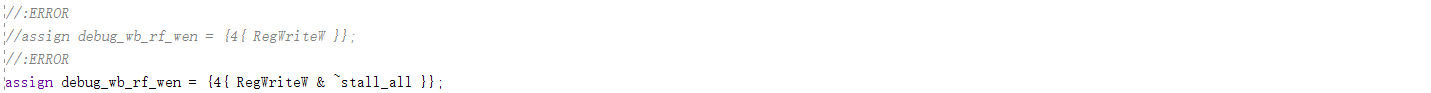
\includegraphics[width=\textwidth]{image/错误5-修正效果1.png}
    \caption{错误5-修正方式}
    \label{fig:错误5-修正效果1}
\end{figure}

\end{enumerate}


\subsubsection{错误6}

\begin{enumerate}[(1)]
    \item 错误现象

在 AXI 功能测试的第 77 个测试点(软件中断测试)中,位于地址 0xbfc005d0 的指令

\begin{lstlisting}
bfc005d0:	401a7000 	mfc0	k0,c0_epc
\end{lstlisting}

读出的值错误。

\begin{figure}[H]
    \centering
    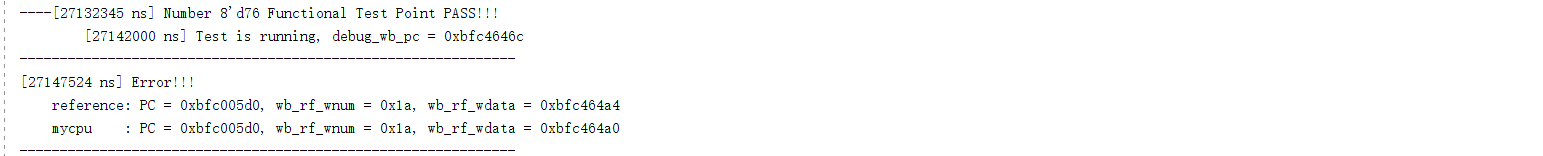
\includegraphics[width=\textwidth]{image/错误6-错误现象1.png}
    \caption{错误6-错误现象}
    \label{fig:错误6-错误现象1}
\end{figure}

    \item 分析定位过程

错误信息中仅 wb\_rf\_wdata 错误。该指令执行的操作是将 CP0 中的 EPC 写入寄存器堆中的 k0 寄存器中,因此推测 EPC 的值错误导致读出的值错误。

将 EPC 和 ExceptTypeM 添加到仿真波形图中,观察到在最近的一次异常发生时,地址 0xbfc464a0 被写入 EPC 中。此时发生的异常类型为软件中断异常,与测试点相符。

\begin{figure}[H]
    \centering
    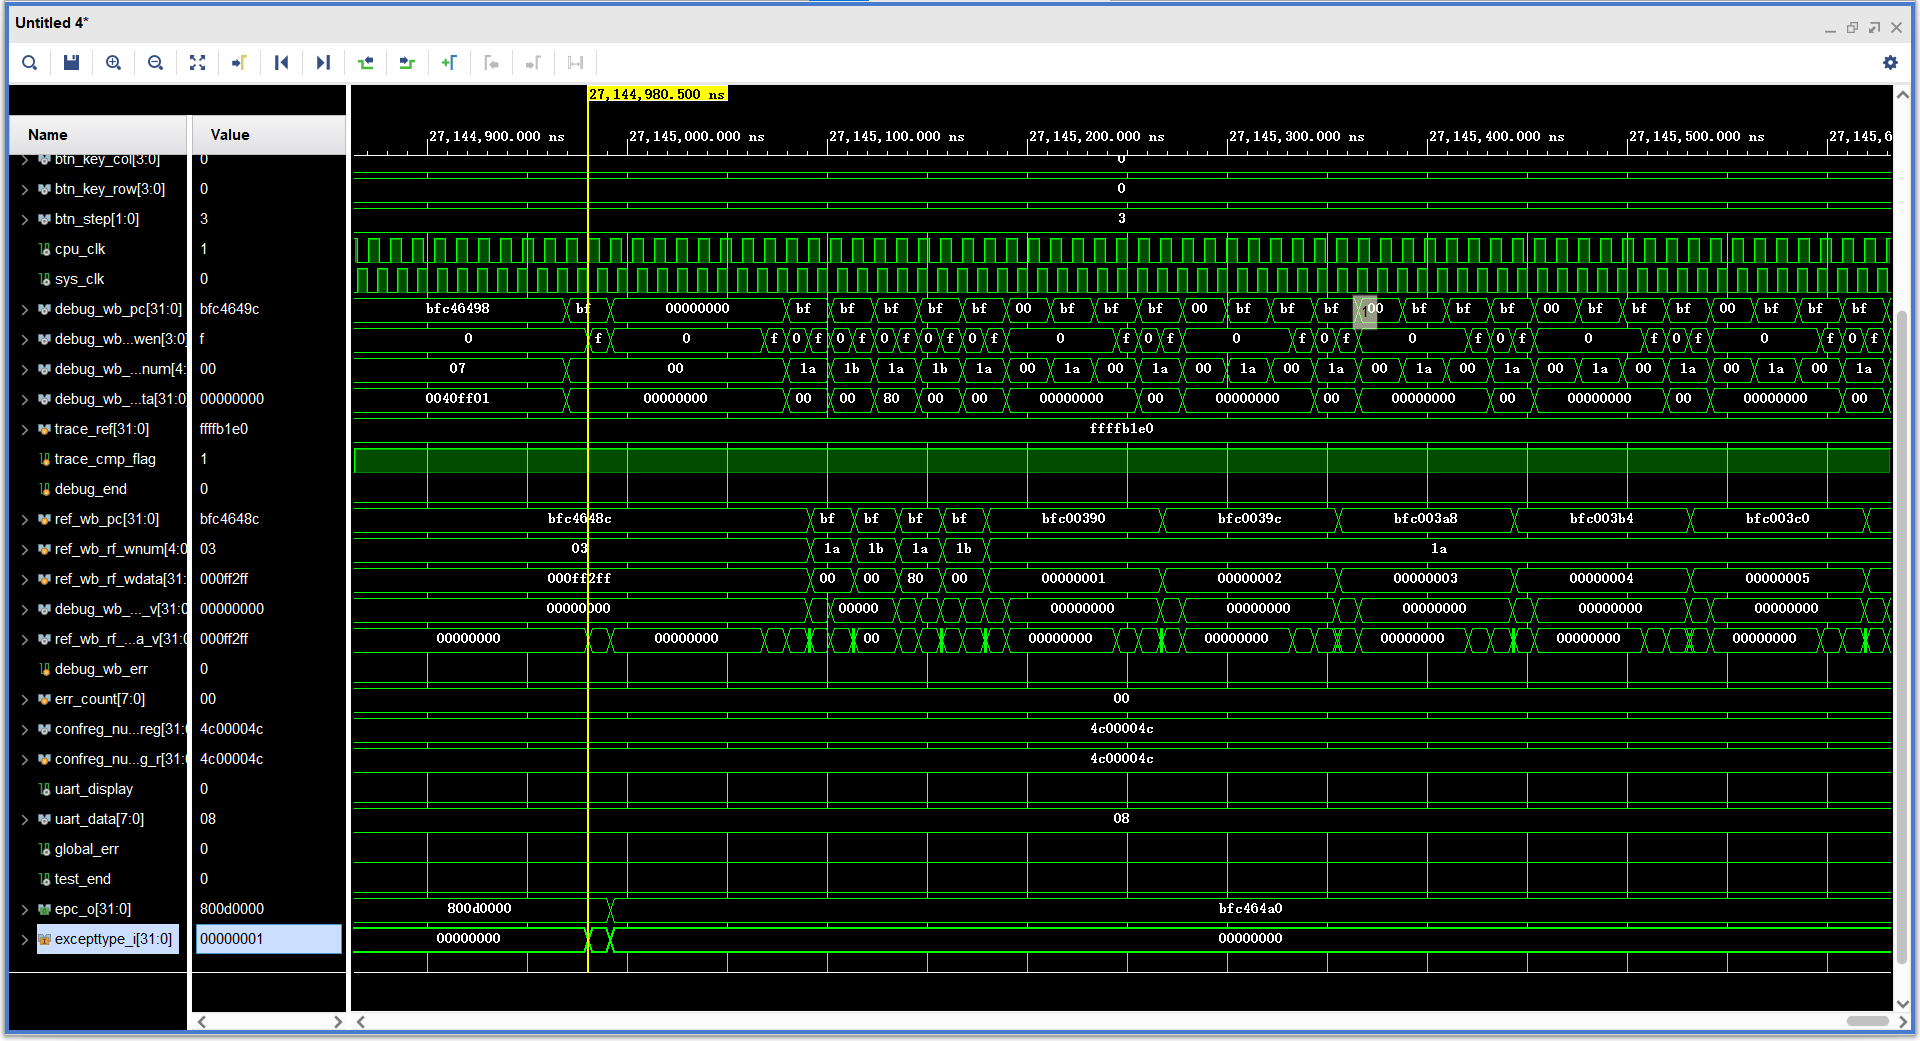
\includegraphics[width=\textwidth]{image/错误6-分析定位过程1.png}
    \caption{错误6-将 ExceptTypeM 添加到仿真波形图}
    \label{fig:错误6-分析定位过程1}
\end{figure}

查找发生软件中断异常的汇编指令(根据仿真波形图可知位于地址 0xbfc4649c 附近)。相关汇编指令为

\begin{lstlisting}
bfc4647c:	3c070040 	lui	a3,0x40
bfc46480:	34e7ff01 	ori	a3,a3,0xff01
...
bfc46488:	3c03000f 	lui	v1,0xf
bfc4648c:	3463f2ff 	ori	v1,v1,0xf2ff
...
bfc46498:	40876000 	mtc0	a3,c0_sr
bfc4649c:	00000000 	nop
bfc464a0:	40836800 	mtc0	v1,c0_cause
\end{lstlisting}

结合软件中断的触发条件(软件中断仅由 Status 寄存器和 Cause 寄存器确定),可以判断这些汇编指令的含义是:通过 MTC0 指令向 Status 寄存器和 Cause 寄存器中写入指定数值,从而构造软件中断。

写入 EPC 的值本应是异常处理程序执行结束后返回的 PC 值,但此时实际写入 EPC 的值 0xbfc464a0 恰好为 MTC0 指令的地址,但是它不应被写入 EPC 中。

结合指令执行过程和相关的数据通路图分析造成错误的原因。在执行到指令

\begin{lstlisting}
bfc464a0:	40836800 	mtc0	v1,c0_cause
\end{lstlisting}

时,CPU 在 MEM 阶段将寄存器 v1 中的数据写入 CP0 中的 Cause 寄存器,此时 Cause 寄存器的输出值同步更新并传递给 Except 模块。在 Except 模块中的组合逻辑将 ExceptTypeM 更新为中断类型(0x00000001)并直接输入 CP0 和 Hazard 模块。在下一个时钟上升沿,流水线被刷新,同时此时的 PCM(指令 MTC0 对应的 PC)被写入 EPC。

\begin{figure}[H]
    \centering
    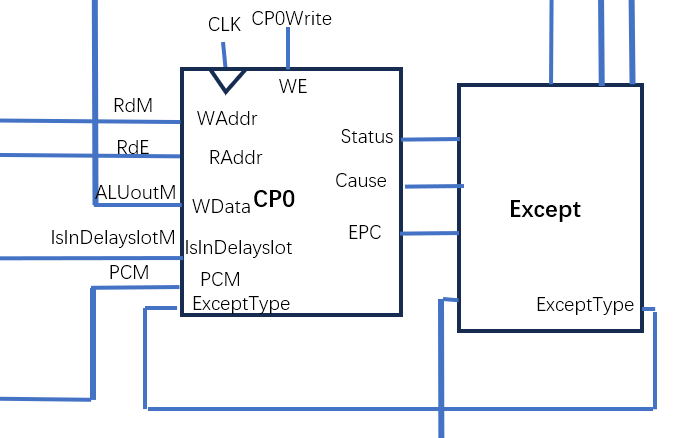
\includegraphics[width=\textwidth]{image/错误6-分析定位过程2.png}
    \caption{错误6-与 CP0 相关的数据通路(含错误)}
    \label{fig:错误6-分析定位过程2}
\end{figure}

以上分析说明原数据通路图的相关部分存在错误,即 CP0 中数据的读和写不可在同一阶段完成。相应的解决方案是将 CP0 中的数据从 EX 阶段读出,通过流水线传递至 MEM 阶段以进行异常处理,这与实验文档中推荐的方式一致。

    \item 错误原因

CP0 的数据读写都在 MEM 阶段完成,导致触发中断异常时写入 EPC 寄存器的返回地址错误。
    
    \item 修正效果

修改原数据通路图,使从 CP0 中读出的数据从 EX 阶段经过流水线传递至 MEM 阶段完成异常处理过程。

\begin{figure}[H]
    \centering
    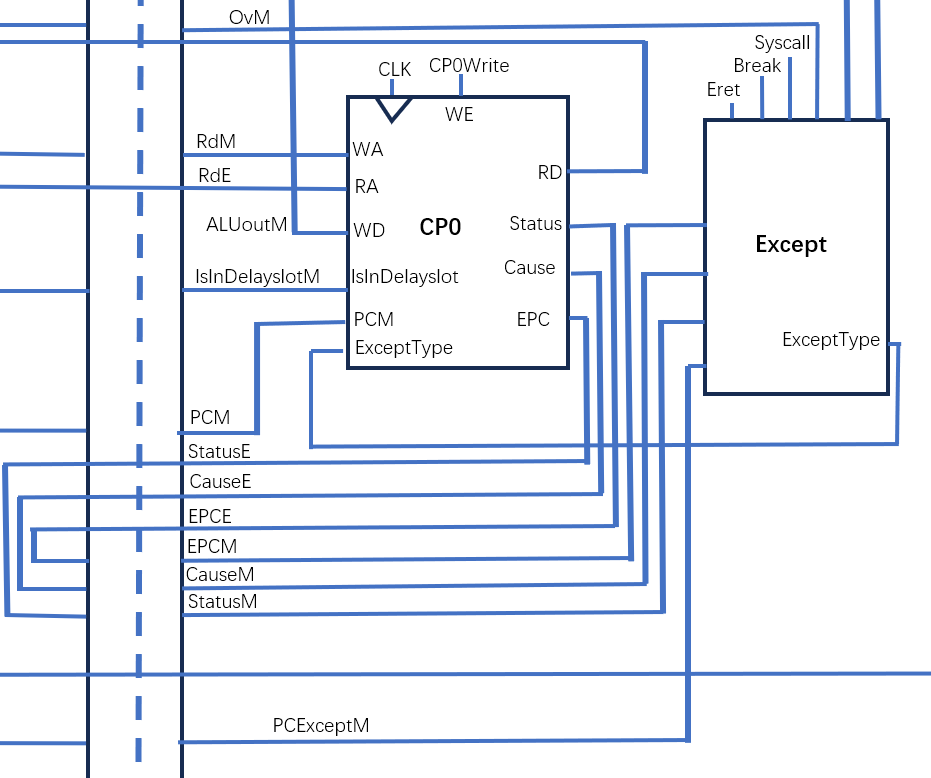
\includegraphics[width=\textwidth]{image/错误6-修正效果1.png}
    \caption{错误6-与 CP0 相关的数据通路(修正后)}
    \label{fig:错误6-修正效果1}
\end{figure}

对代码进行相应的修改。与寄存器堆、HILO 寄存器的读写类似地,对传入 CP0 的时钟信号取反,可以避免数据前推。

\begin{figure}[H]
    \centering
    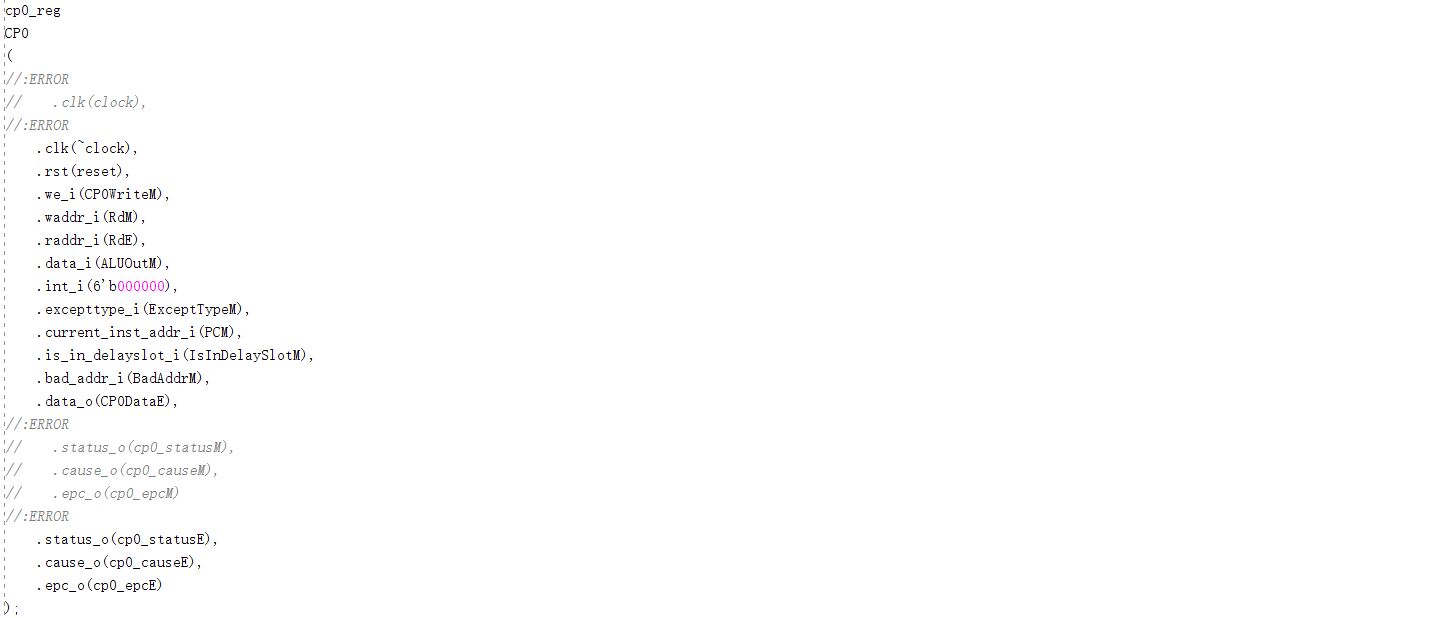
\includegraphics[width=\textwidth]{image/错误6-修正效果2.png}
    \caption{错误6-修正相关代码}
    \label{fig:错误6-修正效果2}
\end{figure}

修改后通过第 77 个测试点。

\end{enumerate}


\subsubsection{错误7}

\begin{enumerate}[(1)]
    \item 错误现象

在性能测试 coremark 中,debug\_wb\_pc 保持 0x9fc08a18 不变,同时 debug\_wb\_wdata 为错误取值。

\begin{figure}[H]
    \centering
    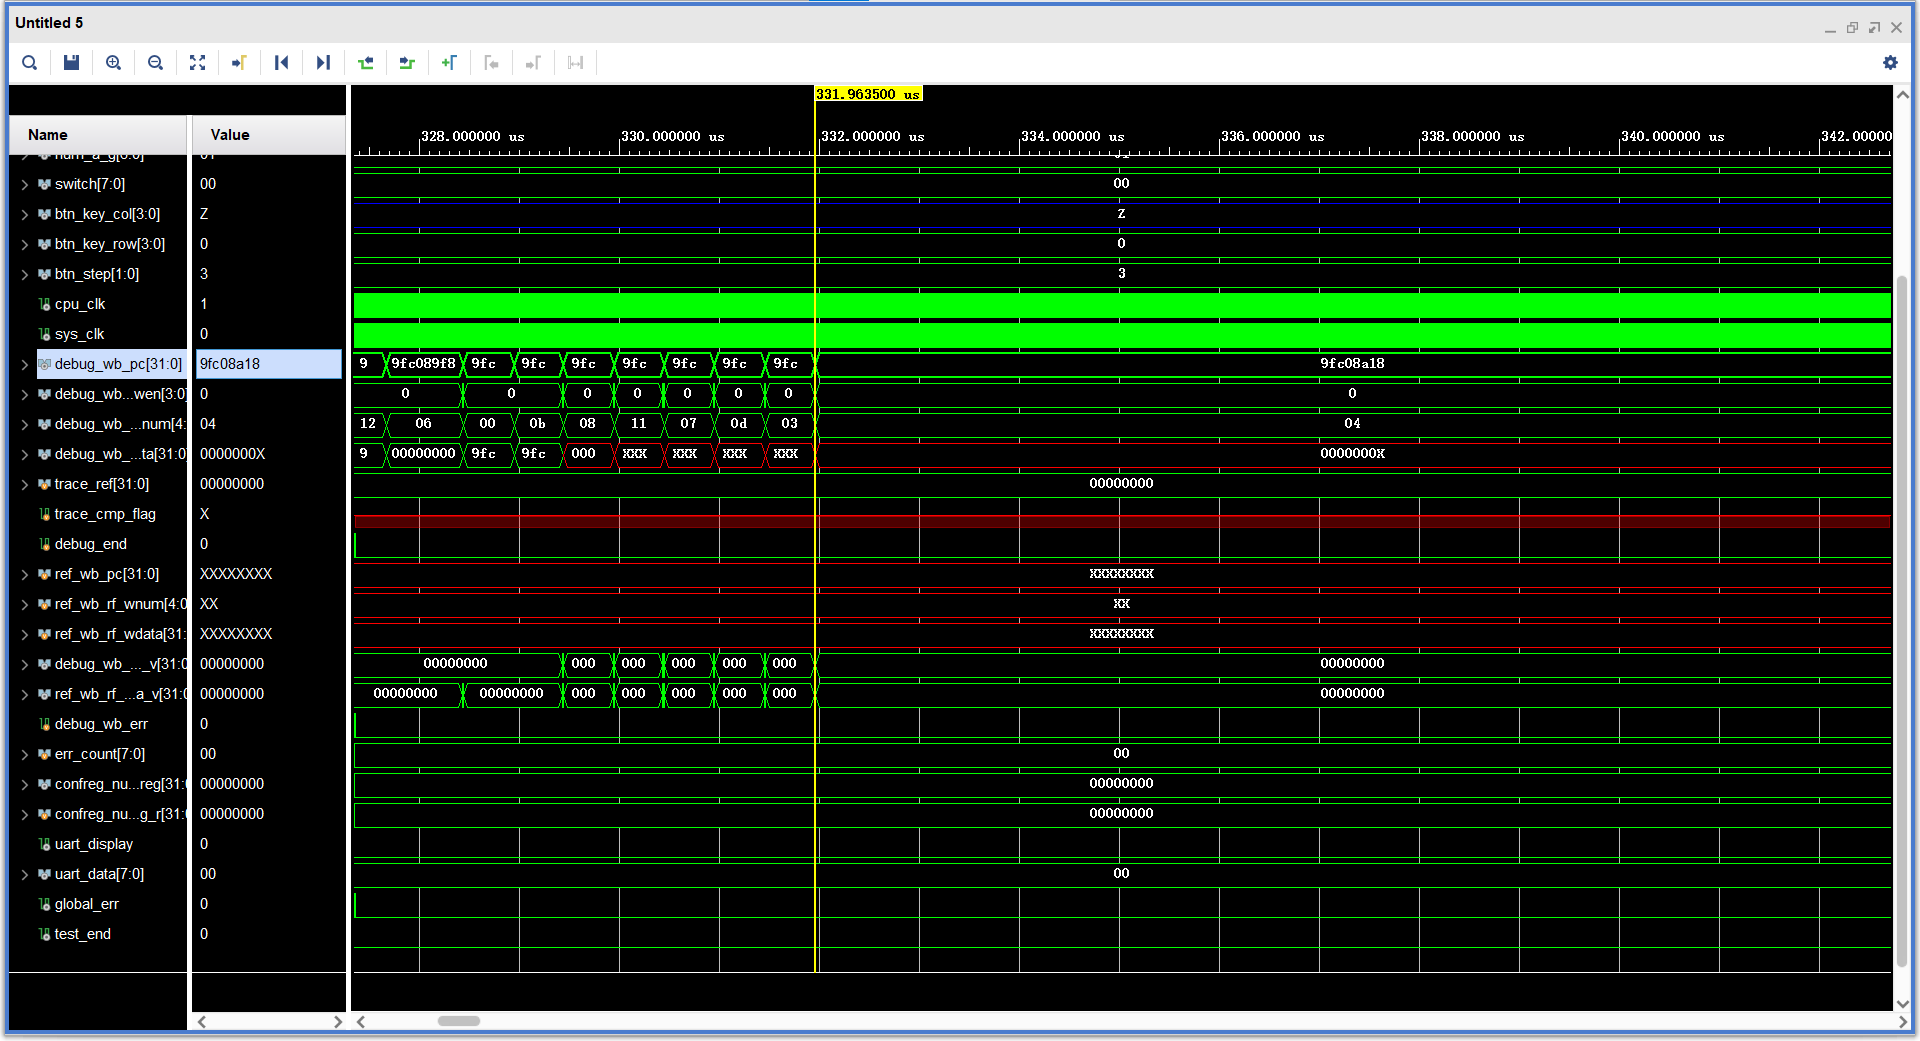
\includegraphics[width=\textwidth]{image/错误7-错误现象1.png}
    \caption{错误7-错误现象}
    \label{fig:错误7-错误现象1}
\end{figure}

    \item 分析定位过程

根据 debug\_wb\_wdata 的错误取值判断程序执行过程中可能存在计算相关错误。追踪其值来源。将与 ALU 计算结果相关的信号添加到仿真波形图中,找到最早导致计算结果错误的 PC 为 0x9fc08a04。对应汇编指令为

\begin{lstlisting}
9fc08a04:	00004012 	mflo	t0
\end{lstlisting}

这说明 HILO 寄存器中的值可能存在错误,因此继续将 HILO 寄存器相关信号添加到仿真波形图中。

\begin{figure}[H]
    \centering
    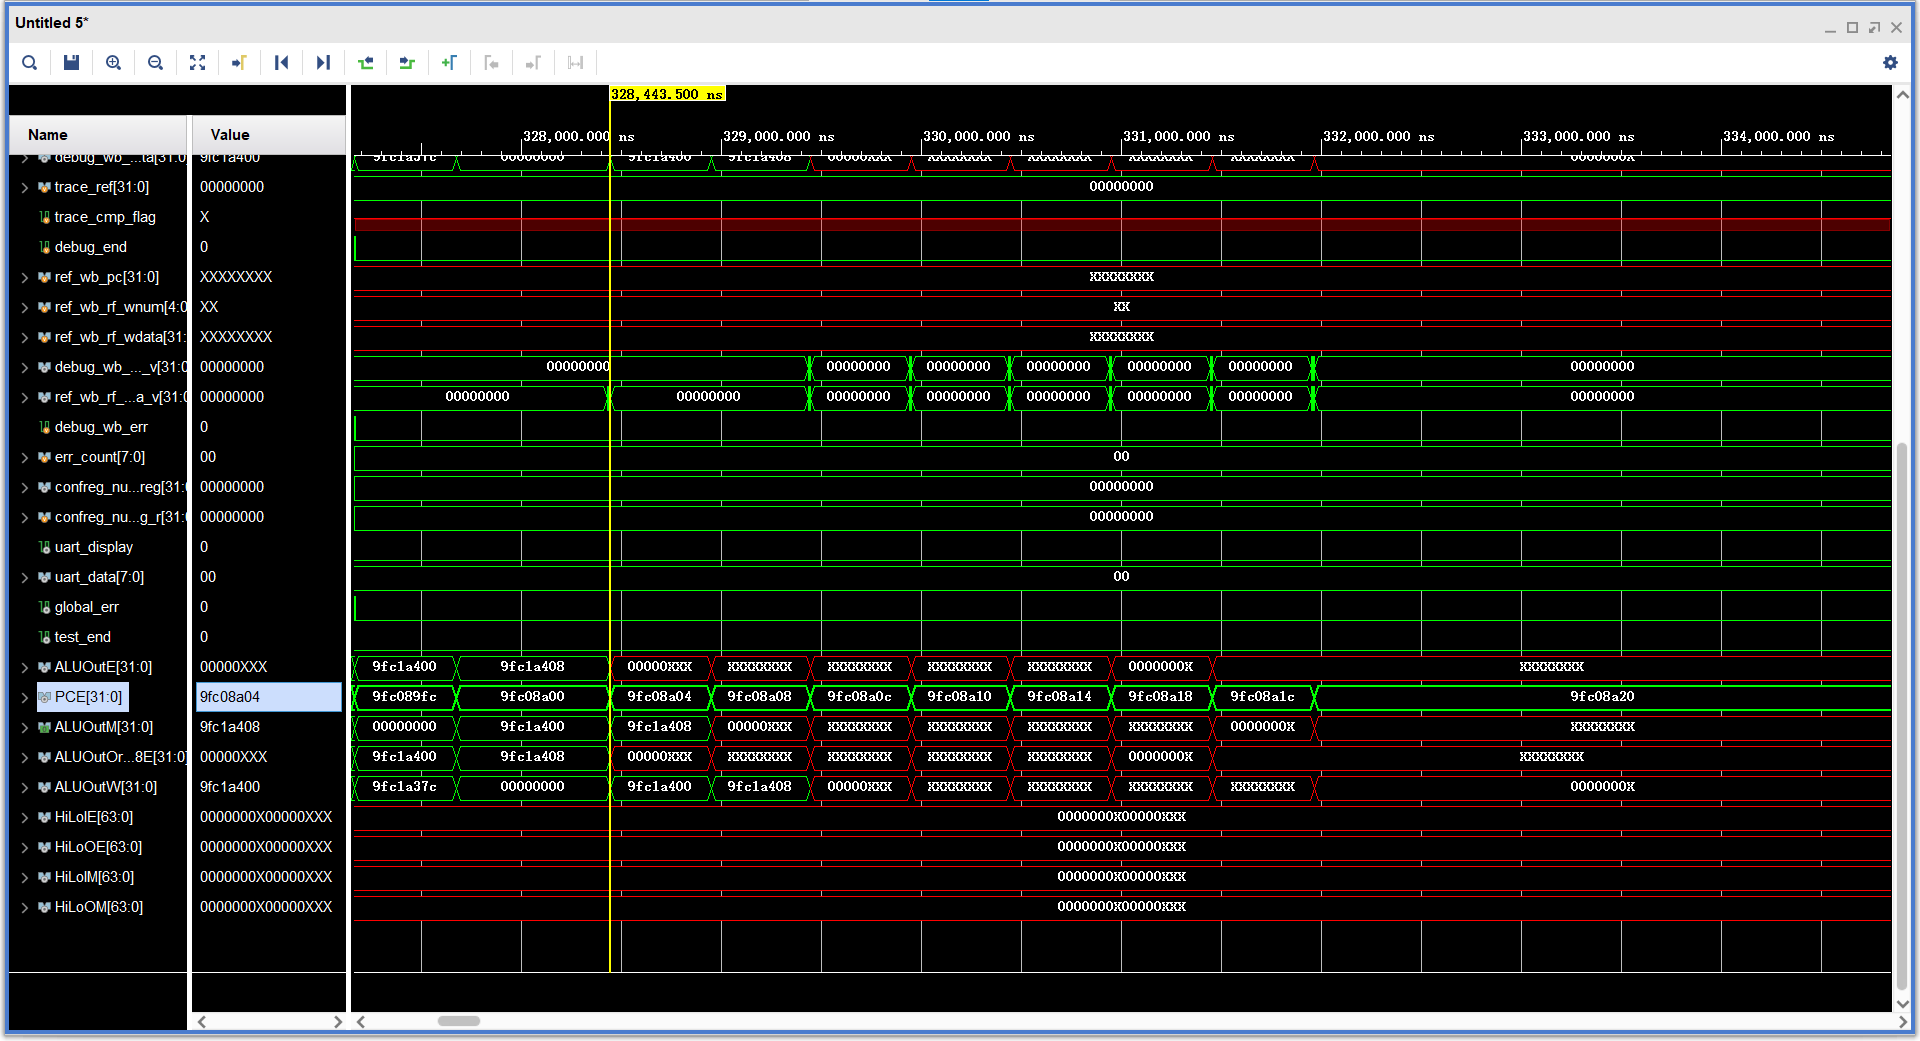
\includegraphics[width=\textwidth]{image/错误7-分析定位过程1.png}
    \caption{错误7-将 HILO 寄存器相关信号添加到仿真波形图中}
    \label{fig:错误7-分析定位过程1}
\end{figure}

仿真波形图显示 HILO 寄存器中的值错误。沿波形图找到最先导致 HILO寄存器错误的 PC 为 0x9fc00990。

\begin{figure}[H]
    \centering
    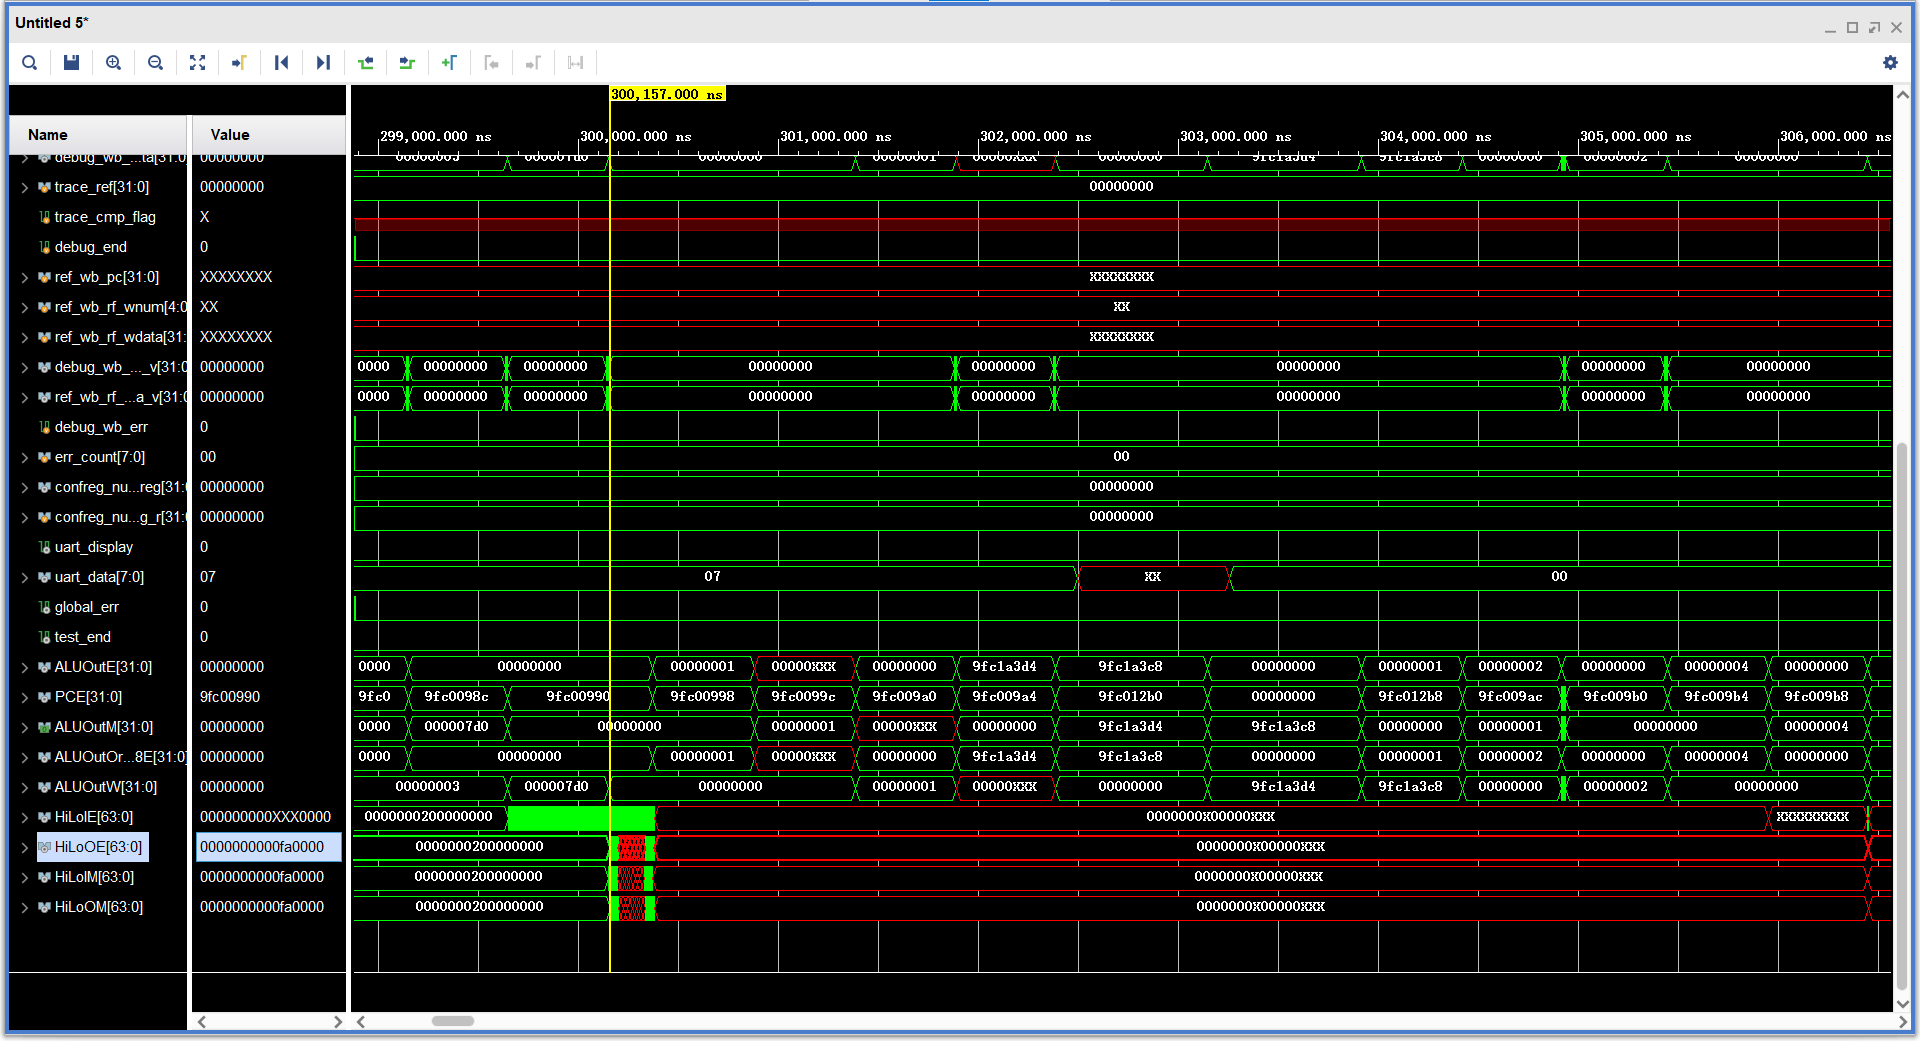
\includegraphics[width=\textwidth]{image/错误7-分析定位过程2.png}
    \caption{错误7-找到最先导致 HILO寄存器错误的 PC}
    \label{fig:错误7-分析定位过程2}
\end{figure}

对应汇编指令为

\begin{lstlisting}
9fc00990:	02af001b 	divu	zero,s5,t7
\end{lstlisting}

在除法运算中,计算的中间结果会直接输出到 HiLoIE 中,使信号呈现持续波动状态,这与仿真波形图中的现象相同,说明该除法运算指令导致错误发生。

阅读与该除法指令相关的汇编指令。

\begin{lstlisting}
9fc00984:	304fffff 	andi	t7,v0,0xffff
9fc00988:	241507d0 	li	s5,2000
9fc0098c:	15e00002 	bnez	t7,9fc00998 <core_mark+0x108>
9fc00990:	02af001b 	divu	zero,s5,t7
9fc00994:	0007000d 	break	0x7
\end{lstlisting}

其中寄存器 t7 的值难以通过汇编指令判断,因此需要通过其他方式理解代码的含义。

注意到 DIVU 指令后紧跟着 BREAK 指令,因此将 ExceptTypeM 添加到仿真波形图中,观察到此时未发生异常。

\begin{figure}[H]
    \centering
    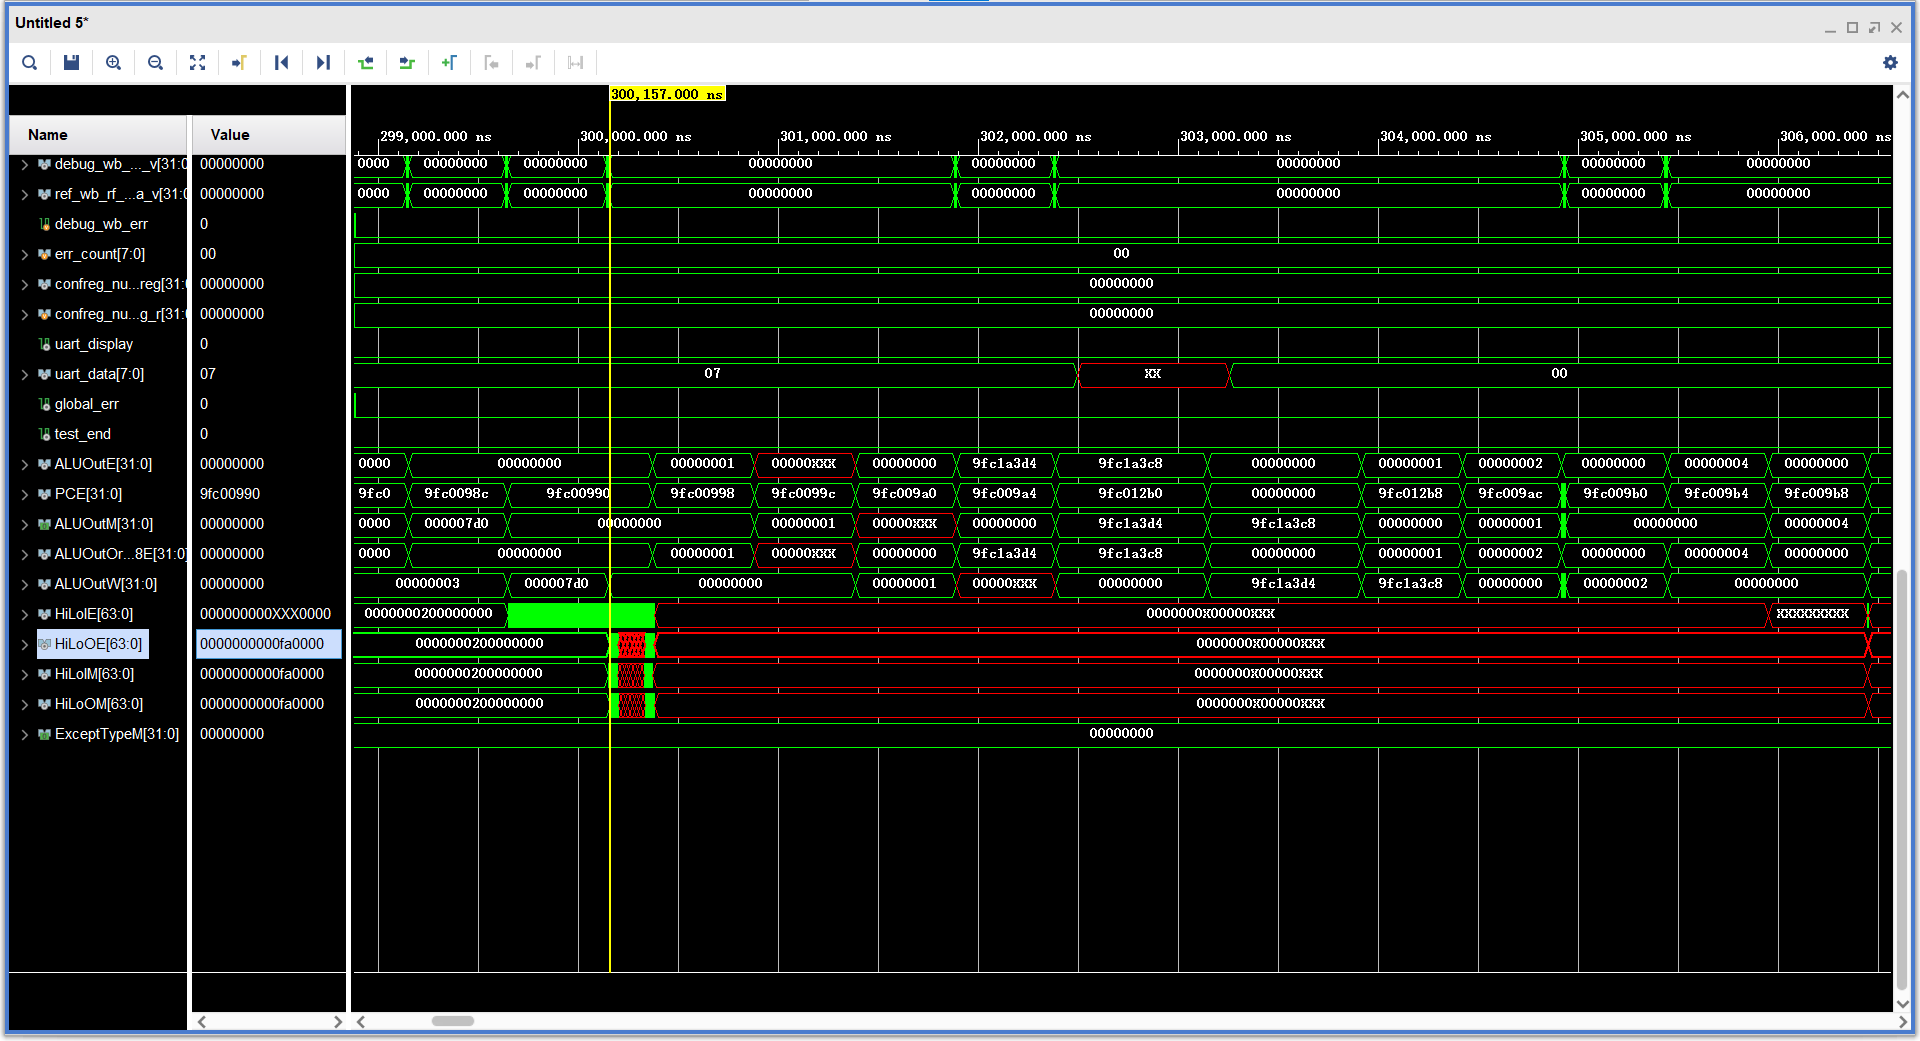
\includegraphics[width=\textwidth]{image/错误7-分析定位过程3.png}
    \caption{错误7-出错时 ExceptTypeM 始终为 0 说明 BREAK 指令未执行}
    \label{fig:错误7-分析定位过程3}
\end{figure}

这说明 BREAK 指令未执行。推测 BNEZ 指令将跳转到地址 <core\_mark+0x108>。

将与分支指令相关的信号添加到仿真波形图中,观察到位于地址 0x9fc0098c 的 BNEZ 指令确实跳转了。

\begin{figure}[H]
    \centering
    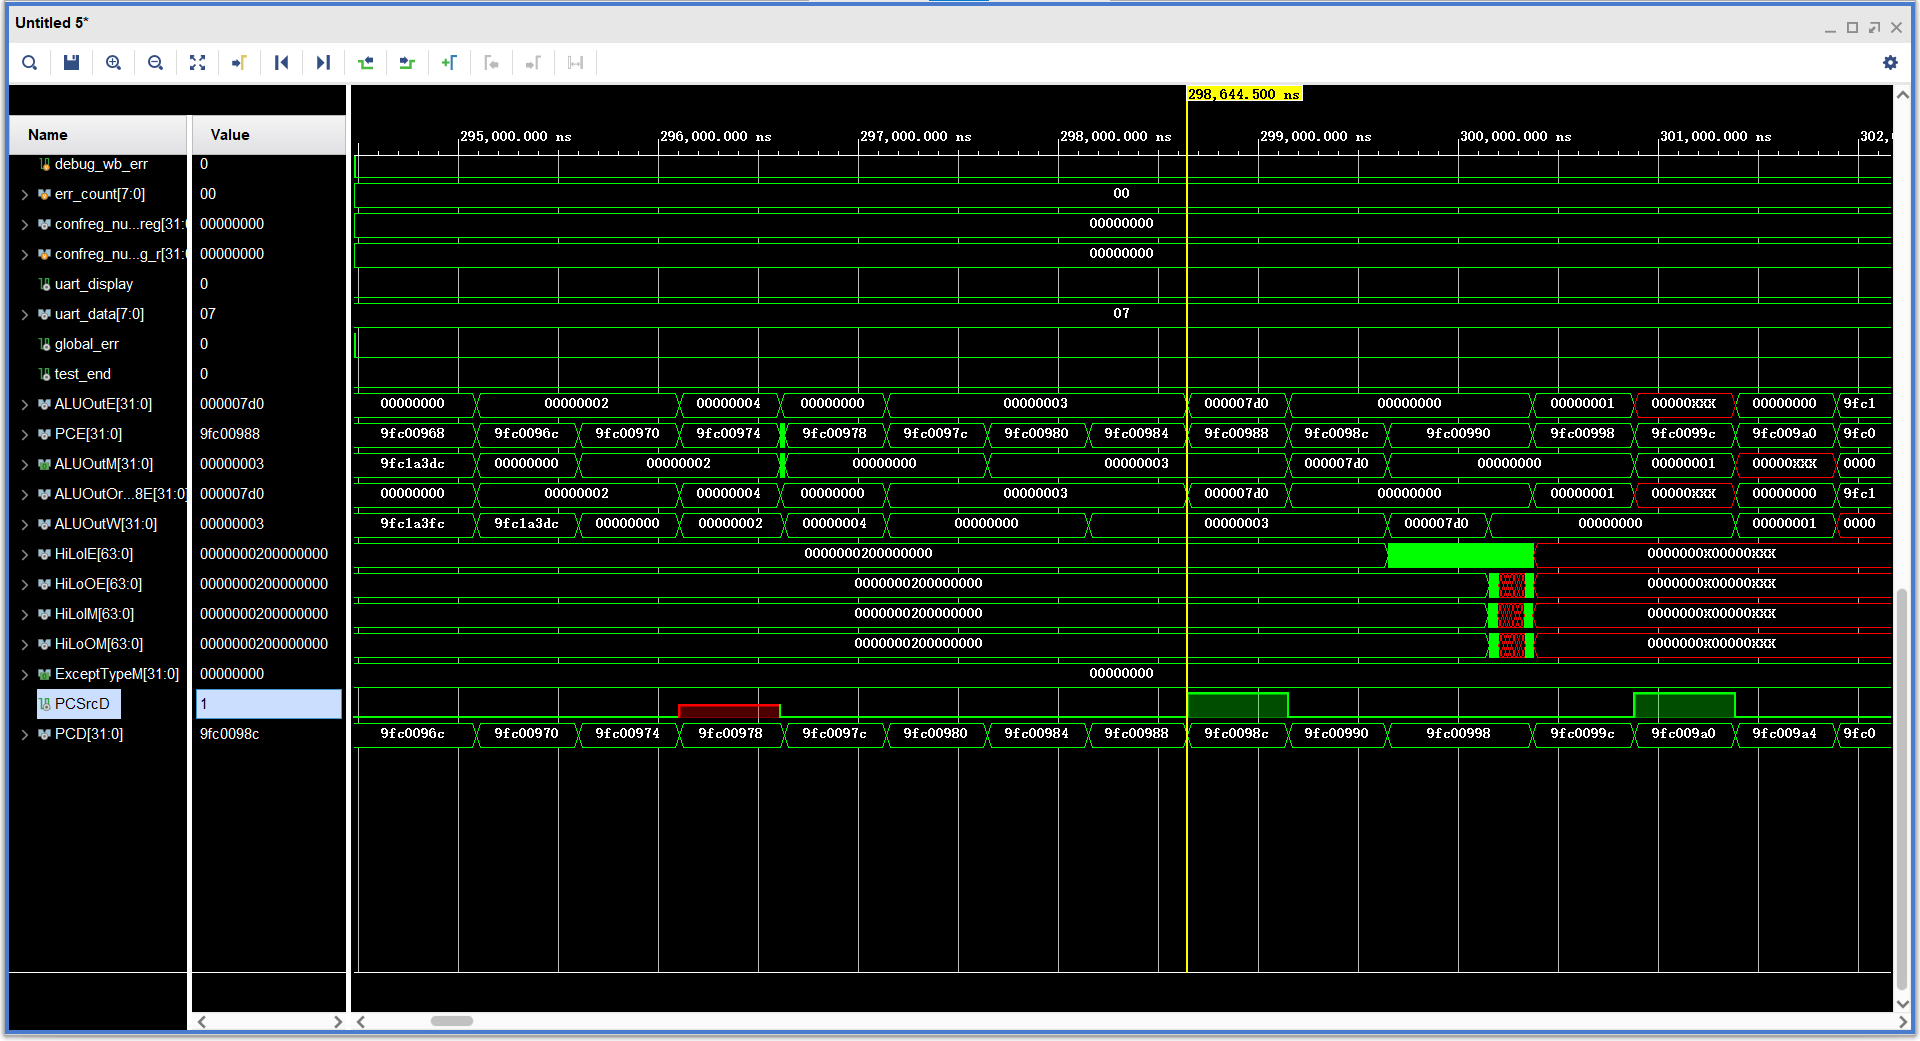
\includegraphics[width=\textwidth]{image/错误7-分析定位过程4.png}
    \caption{错误7-仿真波形图显示 BNEZ 指令跳转}
    \label{fig:错误7-分析定位过程4}
\end{figure}

根据程序执行的逻辑,跳转后 DIVU 指令不应该执行。这里除法运算执行的原因是它恰好在 BNEZ 指令后延迟槽内,而 BNEZ 与 DIVU 之间没有空指令 NOP。要解决这个问题,应阻止 ALU 的运算结果被写入 HILO 寄存器中。

注意到除法指令在 EX 阶段计算过程中,由于i\_stall 和 d\_stall 信号的变化,导致 PCM 和 PCW 改变,而 PCF、PCD 和 PCE 由于除法阻塞而保持不变。同样由于流水线 EX\_MEM 没有被阻塞,导致 HiLoIE 被传入 HiLoIM,进而被写入 HILO 寄存器。据此推测在 Hazard 模块中的除法阻塞信号应当阻塞所有 5 级流水线,而不是仅仅阻塞 PC、IF\_ID、ID\_EX 流水线。

\begin{figure}[H]
    \centering
    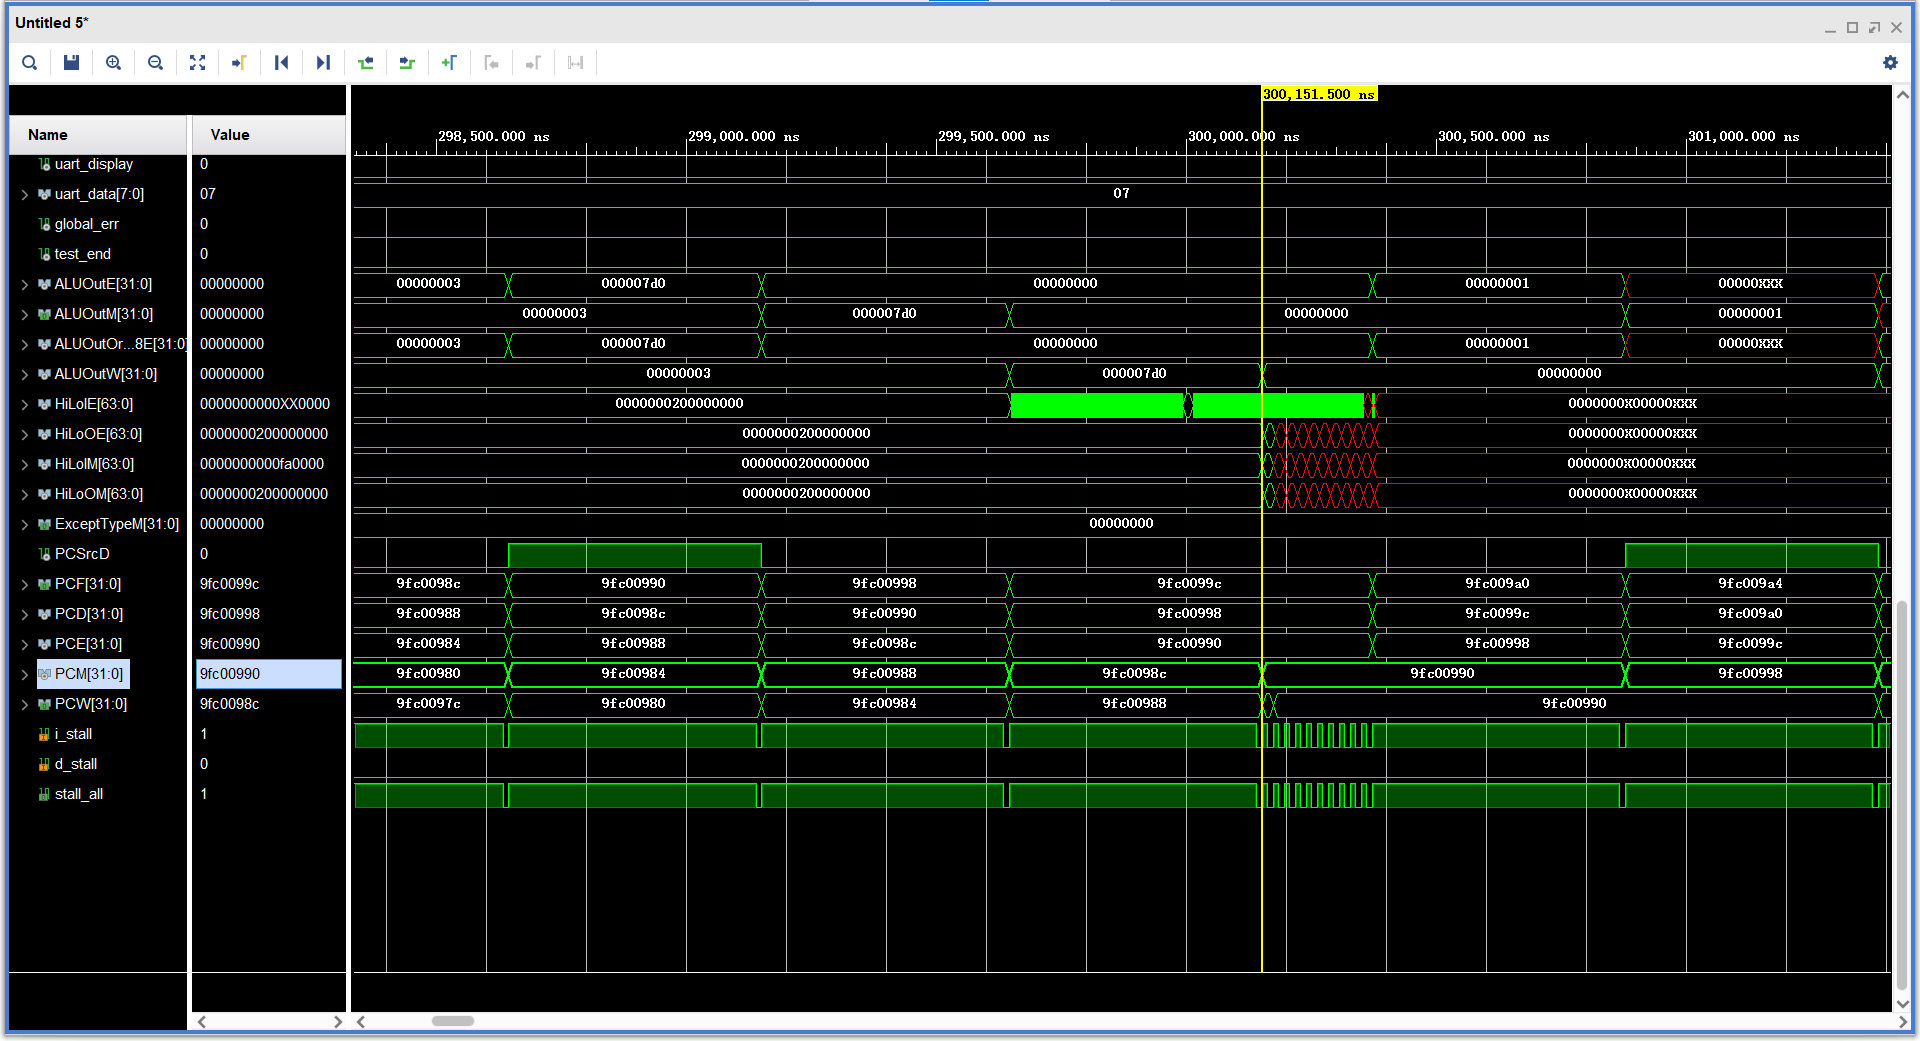
\includegraphics[width=\textwidth]{image/错误7-分析定位过程5.png}
    \caption{错误7-由于 EX\_MEM 流水线未被阻塞导致 HILO 寄存器被修改}
    \label{fig:错误7-分析定位过程5}
\end{figure}

    \item 错误原因

除法阻塞仅仅阻塞了 PC、IF\_ID、ID\_EX 流水线,而未阻塞 EX\_MEM 和 MEM\_WB 流水线;同时在 BNEZ 指令后缺少 NOP 指令,导致 DIVU 不得不执行。二者共同作用导致 HILO 寄存器被修改为错误的值。
    
    \item 修正效果

按图\ref{fig:错误7-修正效果1}所示方式修改将除法阻塞作用于所有 5 级流水线后,解决了此错误,并通过了 coremark 性能测试。

\begin{figure}[H]
    \centering
    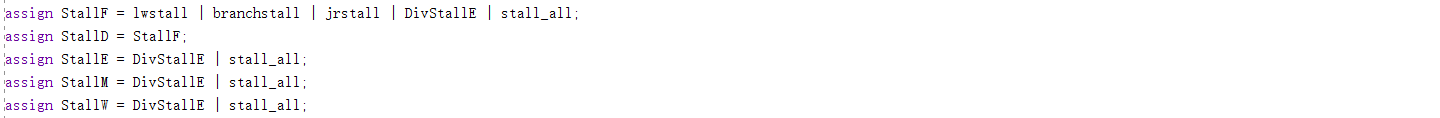
\includegraphics[width=\textwidth]{image/错误7-修正效果1.png}
    \caption{错误7-修正方式}
    \label{fig:错误7-修正效果1}
\end{figure}
    
\end{enumerate}
